%----------------------------------------------------------------------------
%----------------------------------------------------------------------------
%%%%%%%%%%%%%%%%%%%%%%%%%%%%%% -*- Mode: Latex -*- %%%%%%%%%%%%%%%%%%%%%%%%%%%%
%% >>slacT486/intro.tex<<
%% Author          : R. Jeffrey Kowalski
%% Created On      : Tue Apr 10 19:50:51 HST 2007
%% Last Modified On: Thu Aug  2 10:54:56 HST 2007
%%%%%%%%%%%%%%%%%%%%%%%%%%%%%%%%%%%%%%%%%%%%%%%%%%%%%%%%%%%%%%%%%%%%%%%%%%%%%%%
From June 19-24, 2006, the experiment, SLAC T486, was performed in the End Station A facility at the Stanford Linear Accelerator Center to measure the Askaryan effect in ice.  28.5 GeV electrons were accelerated with typically 10$^9$ particles in 10 picosecond bunches and delivered into a 7.5 metric tonne target of carving-grade ice to produce electromagnetic showers.  In a dense media like ice, coherent microwave Cherenkov radiation emerges from the particle shower and propagates to the surface of the target where radio antennas can detect the radiation.  This chapter outlines the T486 experiment and the analysis of the Askaryan effect in ice.
%----------------------------------------------------------------------------
%----------------------------------------------------------------------------
\section{Interaction formalism}
The proposed detection scheme revolves around the laser excitation of a thermal target; i.e. the interaction of a highly prepared optical beam with a relatively unprepared system at equilibrium with ambient conditions. The general equation of motion is derived, the simple example of a two level system subject to a single mode field is examined, and the effects of random orientation and detuning effects are included.
%----------------------------------------------------------------------------
%----------------------------------------------------------------------------
\subsection{General equation of motion}
%----------------------------------------------------------------------------
\label{general dynamics}
%----------------------------------------------------------------------------
%----------------------------------------------------------------------------
%----------------------------------------------------------------------------
Consider an atom which interacts with a multi-mode radiation field. We model the interaction with the minimal-coupling Hamiltonian under the dipole approximation in the radiation gauge \cite{Scully:1997a}:
%----------------------------------------------------------------------------
\begin{equation}
H
=
H_{0}
+
H^{\prime}.
\end{equation}
%----------------------------------------------------------------------------
where $H_0$ is the Hamiltonian of the atomic system, namely
%----------------------------------------------------------------------------
\begin{equation}
H_0 \ket{a}
=
\hbar \omega_a \ket{a}
\end{equation}
%----------------------------------------------------------------------------
where $\ket{a}$ is some energy state of the atom, and $\hbar \omega_a$ is the energy of the state $\ket{a}$; the energy eigenbasis $\{\ket{x}\}$ is assumed complete for electrons bound to the nucleus of the atom (ionization and scattering states are not included here). $H^{\prime}$ is the interaction Hamiltonian, namely
%----------------------------------------------------------------------------
\begin{equation}
H^{\prime}
=
e \vec{E}_n \cdot \vec{r},
\end{equation}
%----------------------------------------------------------------------------
where $e$ is the charge of an electron, $\vec{E}_n$ is the local electric field at the atom due to the nth radiation mode (assumed uniform over the atom), and $\vec{r}$ is the coordinate of the electron (the atomic nucleus is the origin).

If the modes are linearly polarized in the same direction and coherent then the fields can be written as
%----------------------------------------------------------------------------
\begin{equation}
\vec{E}_n
=
\hat{\varepsilon} E_n
\frac
{e^{i (\nu_n t + \phi_n)} - e^{-i (\nu_n t + \phi_n)}}
{2 i}
\end{equation}
%----------------------------------------------------------------------------
where $\hat{\varepsilon}$ is the unit polarization vector for the modes, $E_n$ is the magnitude of the nth mode, $\nu_n$ is the frequency of the nth mode, and $\phi_n$ is the arbitrary phase of the nth mode. Now we can write
%----------------------------------------------------------------------------
\begin{equation}
H^{\prime}
=
\sum_{n}
\frac{1}{2 i}
E_n M
e^{i (\nu_n t + \phi_n)}
+
c.c.
\label{interaction}
\end{equation}
%----------------------------------------------------------------------------
where
%----------------------------------------------------------------------------
\begin{equation}
M\equiv e \hat{\varepsilon} \cdot \vec{r}
\end{equation}
%----------------------------------------------------------------------------
represents the amplitude of the coupling for the nth mode.
%----------------------------------------------------------------------------
%----------------------------------------------------------------------------
%----------------------------------------------------------------------------
%----------------------------------------------------------------------------
%----------------------------------------------------------------------------
%----------------------------------------------------------------------------
%----------------------------------------------------------------------------

The system obeys the Schr\"{o}dinger equation
%----------------------------------------------------------------------------
\begin{equation}
i \hbar \dot{\ket{\psi}}
=
H \ket{\psi}.
\label{raw se}
\end{equation}
%----------------------------------------------------------------------------
If we project the general solution $\ket{\psi}$ into $\{\ket{x}\}$, i.e.
%----------------------------------------------------------------------------
\begin{equation}
\ket{\psi}
=
\sum_a
c_a(t) e^{-i \omega_a t}
\ket{a}
\label{expansion}
\end{equation}
%----------------------------------------------------------------------------
where $c_a(t)$ is the probability amplitude associated with state $\ket{a}$ for $\ket{\psi}$, then Equation \ref{raw se} can be rewritten as \cite{Bransden:1989a}
%----------------------------------------------------------------------------
\begin{equation}
\dot{c_a}
=
\frac{1}{i \hbar}
\sum_b
H^{\prime}_{ab}
e^{(i \omega_{ab} t)}
c_b
\label{se}
\end{equation}
%----------------------------------------------------------------------------
where
%----------------------------------------------------------------------------
\begin{equation}
H^{\prime}_{ab}
=
\bra{a} H^{\prime} \ket{b},
\qquad
\ket{a},\ket{b}
\in
\{\ket{x}\}
\end{equation}
%----------------------------------------------------------------------------
and
%----------------------------------------------------------------------------
\begin{equation}
\omega_{ab}
=
\omega_a - \omega_b
\end{equation}
%----------------------------------------------------------------------------
is the transition energy. Now we combine Equations \ref{interaction} and \ref{se} to obtain the equation of motion for an atom interacting with a multi-mode radiation field:
%----------------------------------------------------------------------------
\begin{equation}
\boxed{
\dot{c_a}
=
\sum_{b,n}
\frac{E_n M_{ab}}{2 \hbar}
(
e^{-i \nu_n t}
-
e^{i \nu_n t}
)
e^{i \omega_{ab} t}
c_b,
\label{dim eom}
}
\end{equation}
%----------------------------------------------------------------------------
where $M_{ab}$ (called the dipole matrix element) is defined as
%----------------------------------------------------------------------------
\begin{equation}
M_{ab}
\equiv
\bra{a} M \ket{b},
\qquad
\ket{a},\ket{b}
\in
\{\ket{x}\}.
\label{matrix element}
\end{equation}
%----------------------------------------------------------------------------
Finally, we introduce
%----------------------------------------------------------------------------
\begin{equation}
\xi
=
\frac
{2 \hbar}
{e E_{o} a_o}
\end{equation}
%----------------------------------------------------------------------------
where $e$ is the elementary charge, $E_{o}$ is an arbitrary constant with units of the electric field, and $a_o$ is the Bohr radius, so that Equation \ref{dim eom} can be written in the dimensionless form (convenient for computer simulations)
%----------------------------------------------------------------------------
\begin{equation}
\frac
{dc_a}
{d\tau}
=
\sum_{b,n}
\Delta_{abn}
(
e^{-i \nu_n \xi \tau}
-
e^{i \nu_n \xi \tau}
)
e^{i \omega_{ab} \xi \tau}
c_b
\label{eom}
\end{equation}
%----------------------------------------------------------------------------
where
%----------------------------------------------------------------------------
\begin{equation}
\Delta_{abn}
=
\xi \frac{E_n M_{ab}}{2 \hbar}
\label{Delta}
\end{equation}
%----------------------------------------------------------------------------
and
%----------------------------------------------------------------------------
\begin{equation}
\tau
=
\frac{t}{\xi}.
\label{tau}
\end{equation}
%----------------------------------------------------------------------------
%----------------------------------------------------------------------------
%----------------------------------------------------------------------------
%----------------------------------------------------------------------------
%----------------------------------------------------------------------------
%----------------------------------------------------------------------------
%----------------------------------------------------------------------------

%----------------------------------------------------------------------------
\subsection{Two level system}
%----------------------------------------------------------------------------
%----------------------------------------------------------------------------
\label{basic_two_level}
%----------------------------------------------------------------------------
%----------------------------------------------------------------------------
If we assume that
%----------------------------------------------------------------------------
\begin{equation}
\omega_b - \omega_a
\neq
\omega_c - \omega_a
\label{condition}
\end{equation}
%----------------------------------------------------------------------------
then pairs of states can be selectively and unambiguously coupled. For real optical beams and real atoms this condition must be generalized to account for laser mode structure/bandwidth and atomic (molecular) transition line widths. Suppose there exists a system in which this is true for at least one transition and consider the simplest example of a single mode field interacting resonantly between the states involved in the transition. Using the rotating wave approximation \cite{Zaheer:1988a} and a single mode with frequency $\nu\equiv\omega_1-\omega_0$, one can show that Equation \ref{eom} reduces to
%----------------------------------------------------------------------------
\begin{subequations}
\begin{eqnarray}
\dot{c_0}
=
-\Delta c_1
\\
\dot{c_1}
=
+\Delta c_0
\end{eqnarray}
\label{two level eom}
\end{subequations}
%----------------------------------------------------------------------------
where $\Delta\equiv\Delta_{10}=\Delta_{01}$ and $\ket{0},\ket{1}\in\{\ket{x}\}$. Of the two selectively coupled states, state $\ket{0}$ is the ``ground''  (initially occupied), and state $\ket{1}$ is the targeted excited state (initially unoccupied).

The solution to Equation \ref{two level eom} can be written as
%----------------------------------------------------------------------------
\begin{equation}
P_1(\tau)
=
\sin^2(\Delta\cdot\tau)
\label{2 level dynamics}
\end{equation}
%----------------------------------------------------------------------------
where $P_1(\tau)\equiv|c_1|^2$ is the probability of finding the system in the excited state $\ket{1}$. When $\Delta\cdot\tau=\pi/2$ the probability of finding the system in $\ket{1}$ is unity, thus whatever portion of the ensemble which was in $\ket{0}$ at $\tau=0$ will be in $\ket{1}$ when $\tau$ satisfies $\Delta\cdot\tau=\pi/2$. It is convenient to define a ``Rabi'' frequency associated with the dynamics described by Equation \ref{two level eom}; in the literature the ``Rabi'' frequency is defined as the angular frequency associated with one complete oscillation (twice the angular frequency associated with the argument of the sine function in Equation \ref{2 level dynamics} since it is squared) or
%----------------------------------------------------------------------------
\begin{equation}
\Omega_R
\equiv
2\frac{
\Delta
}{\xi}
=
\frac{
E_n M_{ab}
}{
\hbar}.
\end{equation}
%----------------------------------------------------------------------------
Now Equation \ref{2 level dynamics} becomes
%----------------------------------------------------------------------------
\begin{equation}
\boxed{
P_1(t)
=
\sin^2
\left(
\frac{\Omega_R}{2}t
\right)
\label{2 level dynamics normal}
}
\end{equation}
%----------------------------------------------------------------------------
where $t$ is in seconds.

Next we seek to derive a relationship between parameters of a tophat pulse with electric field amplitude $E$ and duration $t$ and the resulting fluence when given a specific value of $\Delta \tau$ (usually $\pi/2$). From Equations \ref{Delta} and \ref{tau} we see that the electric field provided by the pulse satisfies
%----------------------------------------------------------------------------
\begin{equation}
E
=
\frac
{(\Delta\tau) 2 \hbar
}{
Mt}
\end{equation}
%----------------------------------------------------------------------------
where $E\equiv E_0$ is the electric field associated with the single mode in this example; thus, the fluence required is
%----------------------------------------------------------------------------
\begin{equation}
\boxed{
f
=
2 c \hbar^2\epsilon_o
(\Delta\tau)^2
\frac{1}{M^2 t}
\label{required fluence}
}
\end{equation}
%----------------------------------------------------------------------------
where $\epsilon_o$ is the permittivity of free space. When only considering the final state of the two level system, it can be shown \cite{Allen:1987a} that the \emph{area} under the amplitude (not intensity) profile of the pulse determines the final state; thus, for a given desired final state, we may concern ourselves with only the total energy contained in the pulse used to excite the system and ignore the exact shape of the profile. Hence, Equation \ref{required fluence} is valid regardless of the pulse shape (even though it was derived for a tophat).
%----------------------------------------------------------------------------
%----------------------------------------------------------------------------
%----------------------------------------------------------------------------
%----------------------------------------------------------------------------

%----------------------------------------------------------------------------
\subsection{Semi-classical behavior of a randomly oriented ensemble}
%----------------------------------------------------------------------------
%----------------------------------------------------------------------------
\label{polarization damping}
%----------------------------------------------------------------------------
Suppose there exists an ensemble of molecules in which we can assign a classical dipole moment to each molecule. Let an incident beam of coherent linearly polarized light interact with each molecule through its dipole moment such that the coupling strength is proportional to $\hat{p} \cdot \hat{\varepsilon}$ where $\hat{p}$ is the direction of the dipole moment and $\hat{\varepsilon}$ the direction of the beam polarization. If the system is unprepared, i.e. we assume it is in thermodynamic equilibrium with its surroundings, the ``orientation polarization'' of the system will be completely incoherent.

Specifically, the normalized dipole vectors of the molecules will be uniformly distributed on the surface of the unit sphere and hence the projections of these vectors against the polarization axis of the incident light are also uniformly distributed. Thus, since the dipole interaction depends linearly on this projection, the distribution of coupling strengths in the ensemble will be uniformly distributed between zero and the maximum case (when the polarization and the dipole moment vectors point in the same direction).

%----------------------------------------------------------------------------
%----------------------------------------------------------------------------
%bb defines the bounding box for the pdf
%viewport defines the area of the pdf used
%in sidewaysfigure the last entry in bb moves the caption toward/away the pic
%in sidewaysfigure the second entry in bb moves the pic toward/away the caption
%----------------------------------------------------------------------------
\begin{figure}
\scalebox{0.8}[0.8]{
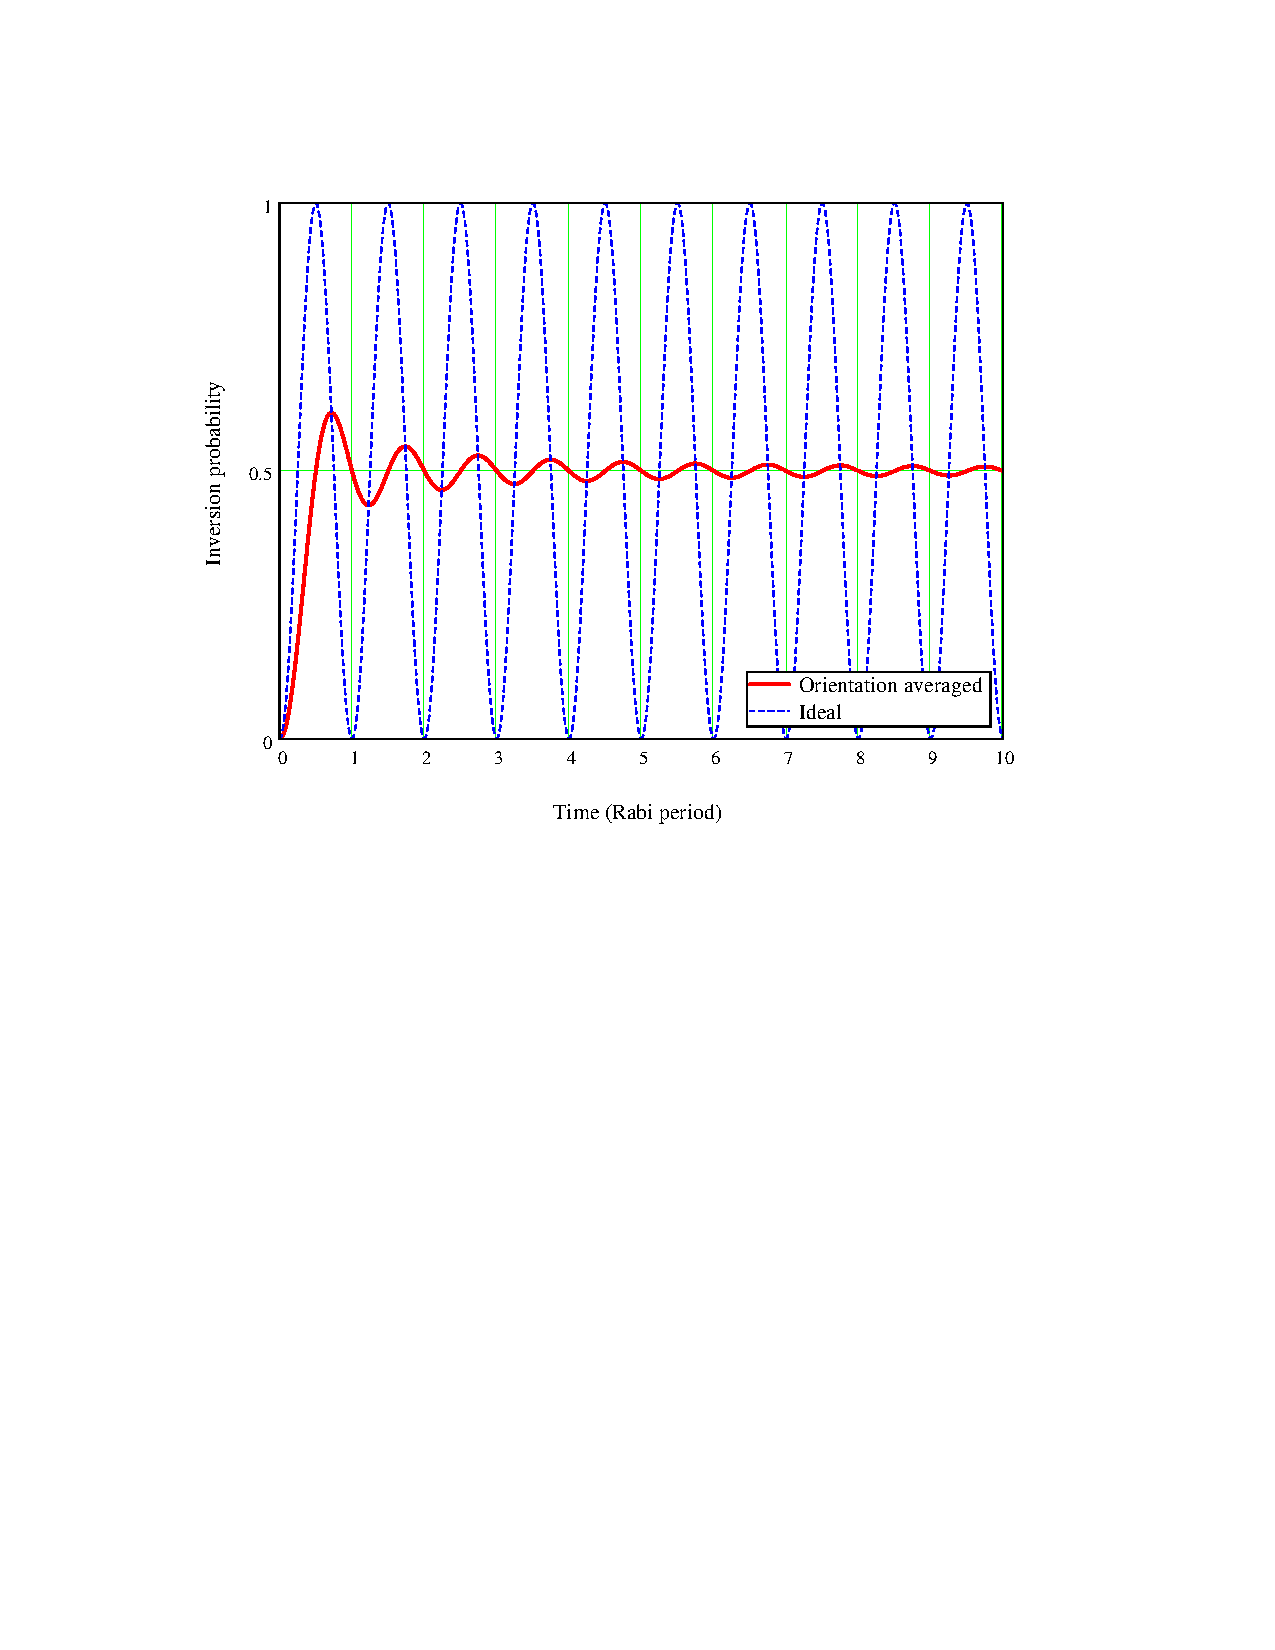
\includegraphics[bb=40 400 489 652]
{dynamics/dynamics.pdf}
}
\caption[Semi-classical behavior of a randomly oriented ensemble]{Semi--classical behavior of a randomly oriented ensemble. Equation \ref{2 level dynamics} is shown as the ``ideal'' behavior while the semi--classical result, Equation \ref{initial eom}, is called ``orientation averaged''.}
\label{dynamics}
\end{figure}
%----------------------------------------------------------------------------

%----------------------------------------------------------------------------
%bb defines the bounding box for the pdf
%viewport defines the area of the pdf used
%in sidewaysfigure the last entry in bb moves the caption toward/away the pic
%in sidewaysfigure the second entry in bb moves the pic toward/away the caption
%----------------------------------------------------------------------------
\begin{figure}
\scalebox{0.8}[0.8]{
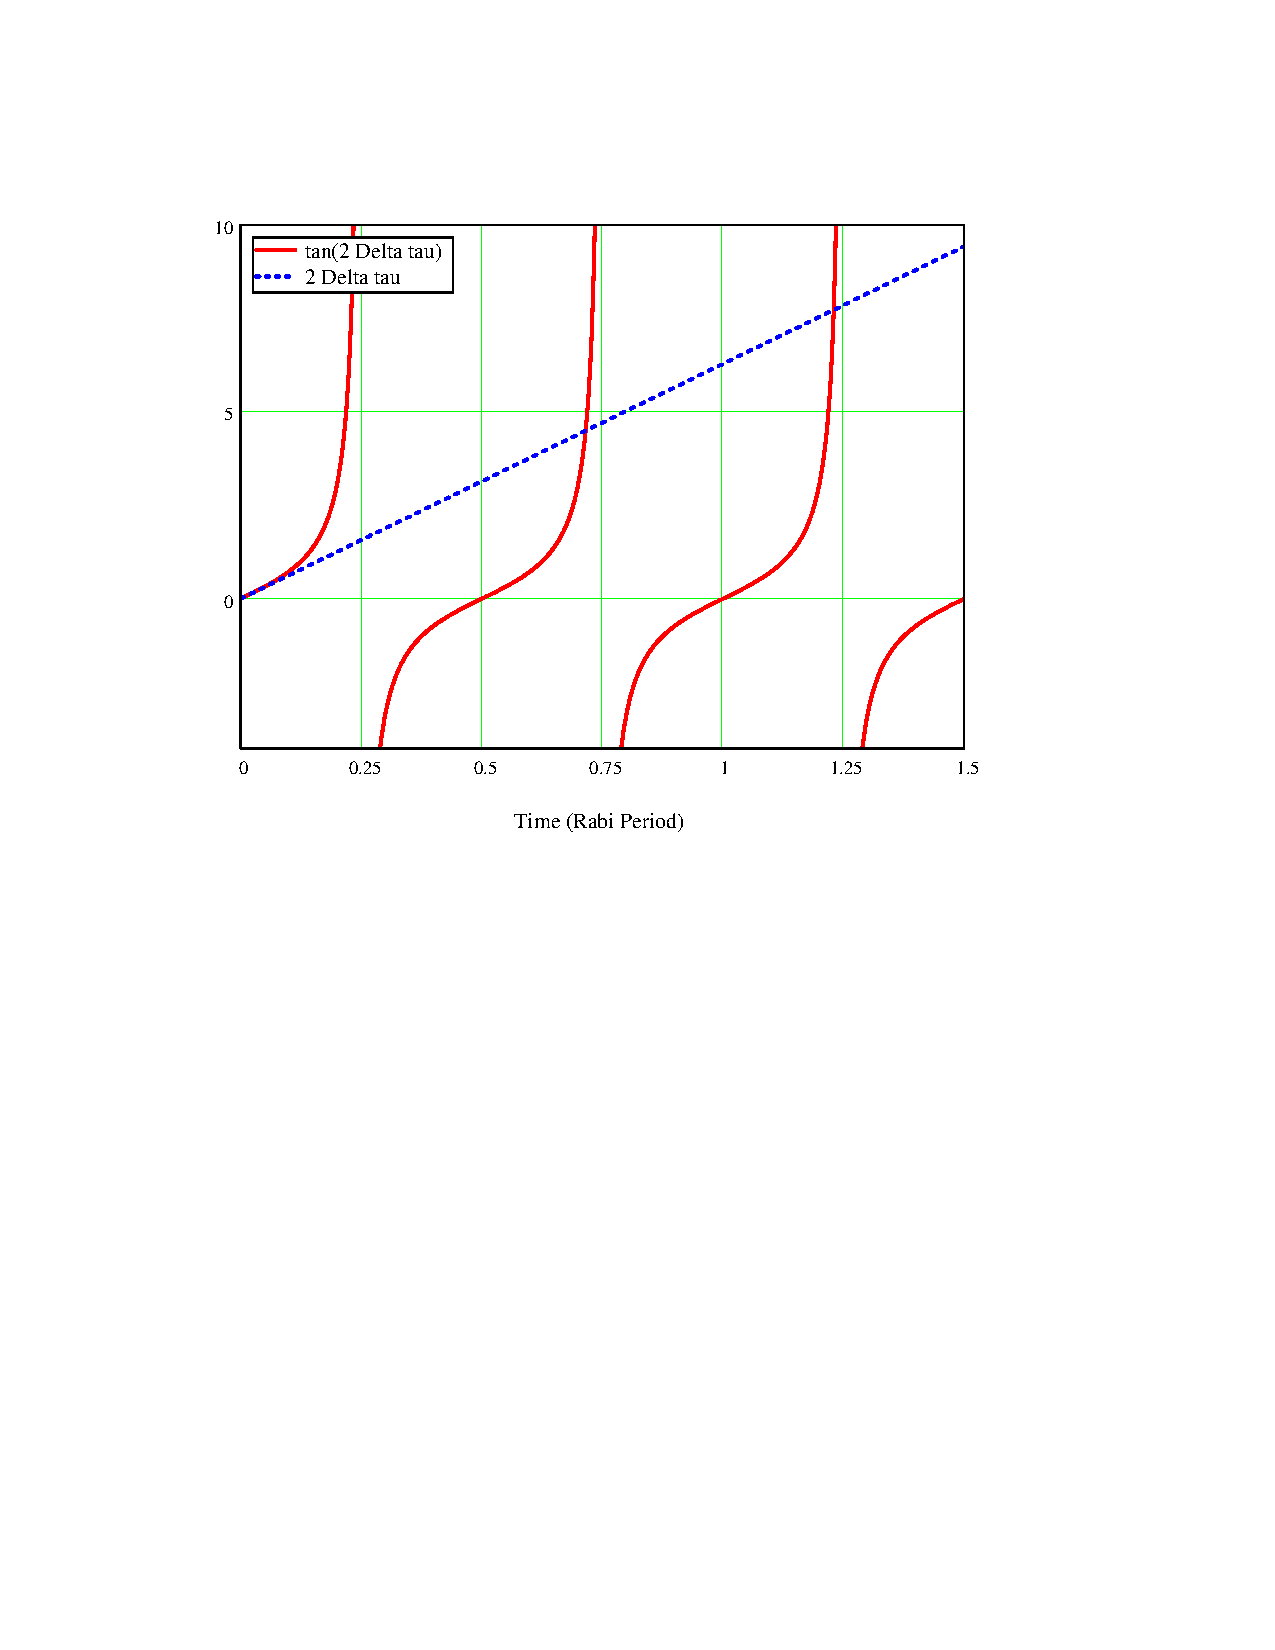
\includegraphics[bb=20 400 489 690]
{extremum/extremum.pdf}
}
\caption[Extremum of the orientation averaged dynamics]{Extremum of the averaged dynamics. The two intersections shown here represent the first absolute maxim and first local minim of the semi--classical behavior shown in Figure \ref{dynamics}. The first maximum has moved from 1/2 Rabi period to about 0.715148 Rabi period. The first minium, which ideally occurs at one Rabi period, has moved to about 1.229512 Rabi period.}
\label{extremum}
\end{figure}
%----------------------------------------------------------------------------

%----------------------------------------------------------------------------
Since the frequency of the Rabi oscillations depend linearly on the matrix element, the Rabi frequency is uniformly distributed in the ensemble. Now, for some molecule with a Rabi frequency reduced from the maximum by a factor $F\in[0,1]$, the probability of excitation at time $\tau$
%----------------------------------------------------------------------------
\begin{equation}
P_1(\tau)
=
\sin^2((F\Delta)\cdot\tau)
\end{equation}
%----------------------------------------------------------------------------
Thus, since the distribution is uniform, the average behavior of a (large) ensemble is
%----------------------------------------------------------------------------
\begin{equation}
P^{\prime}(\tau)
=
\int^{1}_{0}
\sin^2(F\Delta\tau)
dF
=
\frac{1}{2}
\left(
1-
\sinc{(2\Delta\tau)}
\right)
\label{initial eom}
\end{equation}
%----------------------------------------------------------------------------
or
%----------------------------------------------------------------------------
\begin{equation}
P^{\prime}(t)
=
\frac{1}{2}
\left(
1-
\sinc{(\Omega_R t)}
\right)
\label{initial eom normal}
\end{equation}
%----------------------------------------------------------------------------
where
%----------------------------------------------------------------------------
\begin{equation}
\sinc{(x)}
\equiv
\frac
{\sin{(x)}}
{x}.
\end{equation}
%----------------------------------------------------------------------------
See Figure \ref{dynamics} for a comparison between the ideal dynamics of a single molecule and the average behavior our thermal ensemble.

By examining the derivative of Equation \ref{initial eom} one finds that the extrema are located at the solutions to
%----------------------------------------------------------------------------
\begin{equation}
2 \Delta \tau
=
\tan{(2 \Delta \tau)}.
\end{equation}
%----------------------------------------------------------------------------
See Figure \ref{extremum} for a plot of the solution. The implications of these results are that more power will be required to induce the molecules to invert within a give time window (due to the forward shift of the maxima) and the resulting inversion probability will be reduced by a factor of $\sim0.6$. It can be shown that this is a worse case scenario (in terms of reduced modulation depth and forward shift of the maxima) when one compares this semi-classical behavior to the behavior resulting from a quantum mechanical treatment of the dipole approximation in the spherical harmonic basis set (personal communication, Pui K. Lam, June 2006).
%----------------------------------------------------------------------------
%----------------------------------------------------------------------------

%----------------------------------------------------------------------------
\subsection{Detuning effects}
%----------------------------------------------------------------------------
\label{doppler section}
%----------------------------------------------------------------------------
Consider the same two level system studied in section \ref{basic_two_level}. If we start with the same assumptions except instead of perfect resonance we allow for a small mismatch between the excitation field and the transition under consideration (i.e. $\nu\sim\omega_1-\omega_2$) we get
%----------------------------------------------------------------------------
\begin{subequations}
\begin{eqnarray}
\dot{c_0}
&=&
-\Delta
e^{i \xi \tau (\delta \omega)}
c_1
\\
\dot{c_1}
&=&
+\Delta
e^{i \xi \tau (-\delta \omega)}
c_0
\end{eqnarray}
\label{doppler eom}
\end{subequations}
%----------------------------------------------------------------------------
where $\delta \omega = \nu\ - (\omega_1-\omega_2)$, $\Delta\equiv\Delta_{10}=\Delta_{01}$, and $\ket{0},\ket{1}\in\{\ket{x}\}$. Of the two selectively coupled states, state $\ket{0}$ is the ``ground'', i.e. initially occupied; and state $\ket{1}$ is the targeted excited state, initially unoccupied.

The solution to \ref{doppler eom} is
%----------------------------------------------------------------------------
\begin{subequations}
\begin{eqnarray}
c_0
&=&
\exp{\left(
i \frac{\Phi}{2} \tau
\right)}
\left(
\cos{\left(
\frac{\Omega}{2} \tau
\right)}
-
i\sin{\left(
\frac{\Omega}{2} \tau
\right)}
\right)
\\
c_1
&=&
\frac{2 \Delta}{\Omega}
\exp{\left(
-i \frac{\Phi}{2} \tau
\right)}
\sin{\left(
\frac{\Omega}{2} \tau
\right)}
\end{eqnarray}
\end{subequations}
%----------------------------------------------------------------------------
where $\Phi \equiv \xi \cdot\delta\omega$ (dimensionless detuning) and $\Omega\equiv \sqrt{\Phi^2 +4\Delta^2}$. Now
%----------------------------------------------------------------------------
\begin{equation}
P_1(\tau)
=
\left( \frac{2 \Delta}{\Omega} \right)^2
\sin^2{\left(
\frac{\Omega}{2} \tau
\right)}
\end{equation}
%----------------------------------------------------------------------------
or
%----------------------------------------------------------------------------
\begin{equation}
P_1(\tau,\Phi)
=
\frac
{1}
{
1+\left(\frac{\Phi}{2\Delta}\right)^2
}
\sin^2{\left(
\Delta \tau \sqrt{1+\left(\frac{\Phi}{2\Delta}\right)^2}
\right)}
\end{equation}
%----------------------------------------------------------------------------
where $P_1(\tau)\equiv|c_1|^2$. This can be rewritten as
%----------------------------------------------------------------------------
\begin{equation}
\boxed{
P_1(t,\delta\omega)
=
\frac
{1}
{
1+\left(\frac{\delta\omega}{\Omega_R}\right)^2
}
\sin^2{\left( 
\frac{\Omega_R}{2} t \sqrt{1+\left(\frac{\delta\omega}{\Omega_R}\right)^2}
\right)}.
\label{final eom}
}
\end{equation}
%----------------------------------------------------------------------------

%----------------------------------------------------------------------------
%----------------------------------------------------------------------------
%bb defines the bounding box for the pdf
%viewport defines the area of the pdf used
%in sidewaysfigure the last entry in bb moves the caption toward/away the pic
%in sidewaysfigure the second entry in bb moves the pic toward/away the caption
%----------------------------------------------------------------------------
\begin{figure}
\scalebox{0.8}[0.8]{
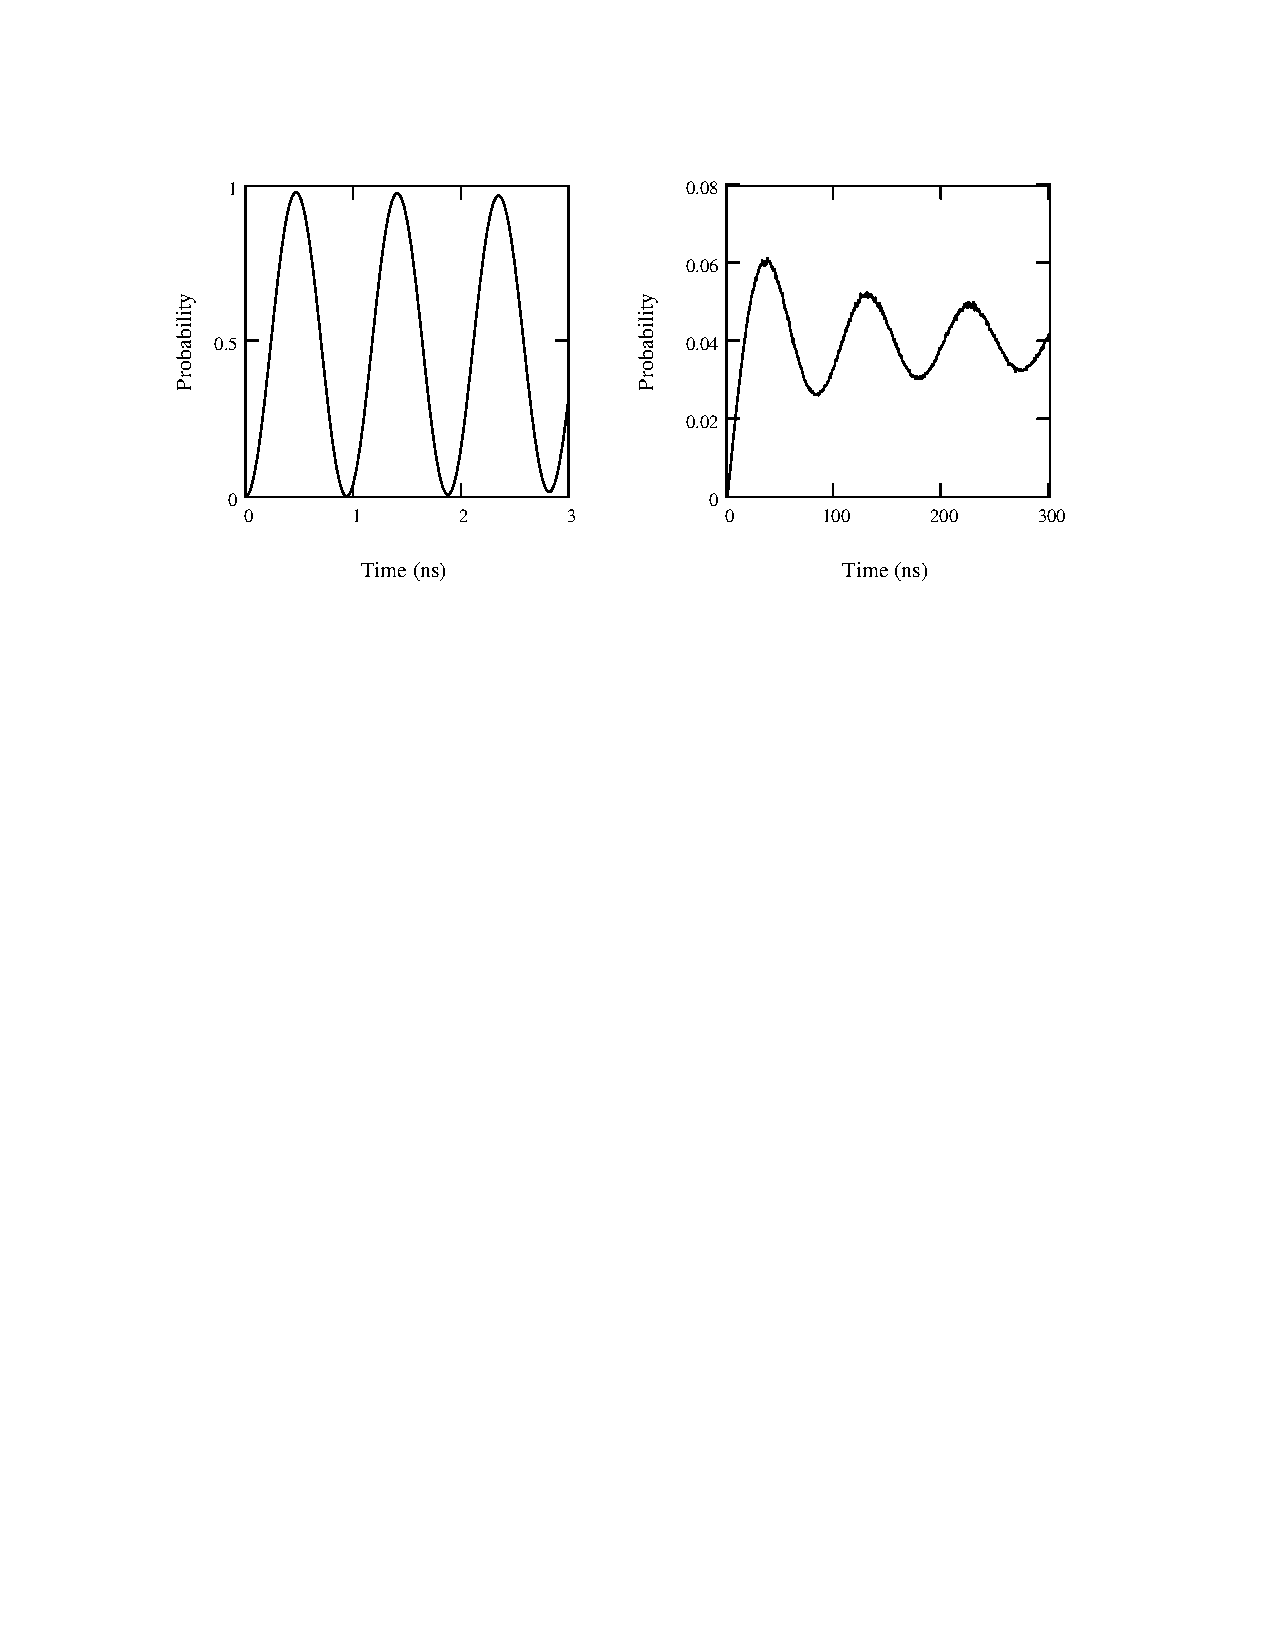
\includegraphics[bb=35 515 550 700]
{doppler_only/doppler_only.pdf}
}
\caption[Simulated thermal (Doppler only) effects on observed fluorescence -- high fluence vs. low fluence]{Simulated thermal (Doppler only) effects on observed fluorescence -- high fluence vs. low fluence. For these two simulations we use a fluence of 1000 J/m$^2$ for the left plot and a fluence of 10 J/m$^2$ for the right plot. The target is thermal molecular iodine gas with dipole matrix element $3.6\cross10^{-32}$ Cm (including FCF), at T = 293 K.}
\label{doppler_only}
\end{figure}
%----------------------------------------------------------------------------

%----------------------------------------------------------------------------
Clearly we would like to work in the limit $\delta\omega/\Omega_R<<1$ (this is equivalent to $\Phi/2\Delta<<1$); unfortunately, this ratio is near unity for ambient atmospheric targets excited with ns laser pulses. $\Omega_R$ must be faster than the relaxation processes in the atmosphere, about 1ns; thus $\Omega_R\sim$1 GHz. $\Delta\omega$ is forced to be at least 0.36 GHz due to Doppler broadening; however, laser line broadening produces an equivalent effect, thus the transform limit of the 1  ns laser pulse will place a lower limit on $\delta\omega$: again about 1 GHz. See Figure \ref{doppler_only} for a comparison between ``fast'' population transfer (using a 2 ns pulse) and a ``slow'' transfer (using a 200 ns pulse).
%----------------------------------------------------------------------------
%----------------------------------------------------------------------------
%----------------------------------------------------------------------------

%----------------------------------------------------------------------------
%----------------------------------------------------------------------------
\section{LIDAR geometries}
For a geometry appropriate for a benchtop demonstration experiment (side view), a computer model is used to explore the effects of phase space constraints of thermal velocities on the photon capture probability. In the last subsection (Section \ref{backscatter section}), a simple geometric argument is applied to general LIDAR systems to place limits on the photon capture probability and quantify the required pulse energies for molecular control.
%----------------------------------------------------------------------------
%----------------------------------------------------------------------------
\subsection{Receiver phase space}
%----------------------------------------------------------------------------
%----------------------------------------------------------------------------
Consider the linear systems of ray optics where rays are traced through a series of optical components \cite{Saleh:1991a}. The rays are assigned two parameters at each position $z$ along the beam line: $x$ (or $y$) which represents the distance from the optic axis and $\alpha$ which represents the angle the ray makes with the optic axis. The rays form vectors in a \emph{phase space} in which their motion down the beam line is modeled; $x$ (or $y$) corresponds to the \emph{position} coordinate while $\alpha$ (which is related to the transverse velocity of the ray) corresponds to the \emph{momentum} coordinate. Optical components such as thin lenses or drift regions (free space regions between lenses) are represented by matrices which can be used to transform any ray to some other position along the beam line. In this study, ``bundles'' of rays are tracked along various beam lines to determine the collection efficiency of two beam line geometries appropriate for LIF investigation.

In terms of the ray optics phase space described above, any receiver in an optical system can be assigned a finite region of phase space to which it is sensitive. This region can be transformed to the target region where it can be overlapped with the phase space of the fluorescence in the target region. The Liouville Theorem \cite{Hassani:1999a} states that the bundle of rays will flow through phase space as an incompressible fluid. This places a fundamental limit to the coupling between the receiver and target region. Suppose the receiver has an acceptance ``half'' angle of 0.07 radians (this was an initial estimate for the monochromator used in the experiments described later in this dissertation). If we assume the spatial extent of the fluorescence is not a limiting factor, then with respect to the angular limits, the Liouville Theorem states that the receiver is sensitive to at most
%----------------------------------------------------------------------------
\begin{equation}
\frac{0.14^2}{4\pi}
=
0.00156
\label{angular overlap}
\end{equation}
%----------------------------------------------------------------------------
or a little over one thousandth of the emitted energy.

Moreover, this phase space overlap, in combination with a molecular density and inversion probability, can be interpreted as a ``photon capture probability'' for the detection system. For example, suppose there were $2\cross10^5$ molecules in the sensitive region and 50\% of the molecules were inverted and decayed optically; then the angular overlap from Equation \ref{angular overlap} implies we should capture 156 photons in our detection system.
%----------------------------------------------------------------------------
%----------------------------------------------------------------------------
%----------------------------------------------------------------------------

%----------------------------------------------------------------------------
\subsection{Monochromator resolution}
%----------------------------------------------------------------------------
%----------------------------------------------------------------------------
The resolution of the 1 m monochromator is calculated from simple assumptions. Suppose monochromatic light is incident on a rectangular slit. The far field diffraction pattern (1 m away) is collimated and sent to a diffraction grating. We assume the significant portion of the illuminated grating completely contains the central maximum of the far field diffraction pattern (squared sinc function). The angular width of the central maximum is given by
%----------------------------------------------------------------------------
\begin{equation}
\theta = 2 \arcsin \left( \frac{\lambda}{a} \right)
\end{equation}
%----------------------------------------------------------------------------
where $\lambda$ is the wavelength of the monochromatic light and $a$ is the width of the slit. Thus, the number of lines illuminated on the grating is (assuming small angles)
%----------------------------------------------------------------------------
\begin{equation}
\kappa
=
L \theta \rho
=
L 2\frac{\lambda}{a} \rho
\end{equation}
%----------------------------------------------------------------------------
where $L$ is the distance between the input slits and the collimating optic and $\rho$ is the groove density of the grating.

The resolving power $R$ of a grating monochromator can be written in terms of the number of illuminated grooves using the Rayleigh criterion \cite{Hecht:1987a}
%----------------------------------------------------------------------------
\begin{equation}
R
=
\frac
{\lambda}
{\Delta \lambda}
=
m \kappa
\label{Rayleigh}
\end{equation}
%----------------------------------------------------------------------------
where $m$ is the diffraction order. Thus
%----------------------------------------------------------------------------
\begin{equation}
\boxed{
R = 2 m L \rho \frac{\lambda}{a}.
\label{resolvance}
}
\end{equation}
%----------------------------------------------------------------------------
For the Interactive Technology CT-103 monochromator $m=1$, $L=1$ m, and $\rho=1200$ lines per mm. The grating in the CT-103 is about 3 7/8'' wide; thus there is an additional constraint on Equation \ref{resolvance}:
%----------------------------------------------------------------------------
\begin{equation}
2 \frac{\lambda}{a}L < 3\frac{7}{8}''.
\end{equation}
%----------------------------------------------------------------------------
For small slit widths (5--50 microns) figure \ref{near_GHz} (\ref{near_cm}) shows the resolution of the CT-103 calculated from Equation \ref{resolvance} for various wavelengths in GHz (inverse cm). Figures \ref{far_THz}, \ref{far_cm}, and \ref{far_nm} show the resolution of the CT-103 for larger slit widths (50--1000 microns).
%----------------------------------------------------------------------------
%----------------------------------------------------------------------------
%bb defines the bounding box for the pdf
%viewport defines the area of the pdf used
%in sidewaysfigure the last entry in bb moves the caption toward/away the pic
%in sidewaysfigure the second entry in bb moves the pic toward/away the caption
%----------------------------------------------------------------------------
\begin{figure}
\scalebox{0.8}[0.8]{
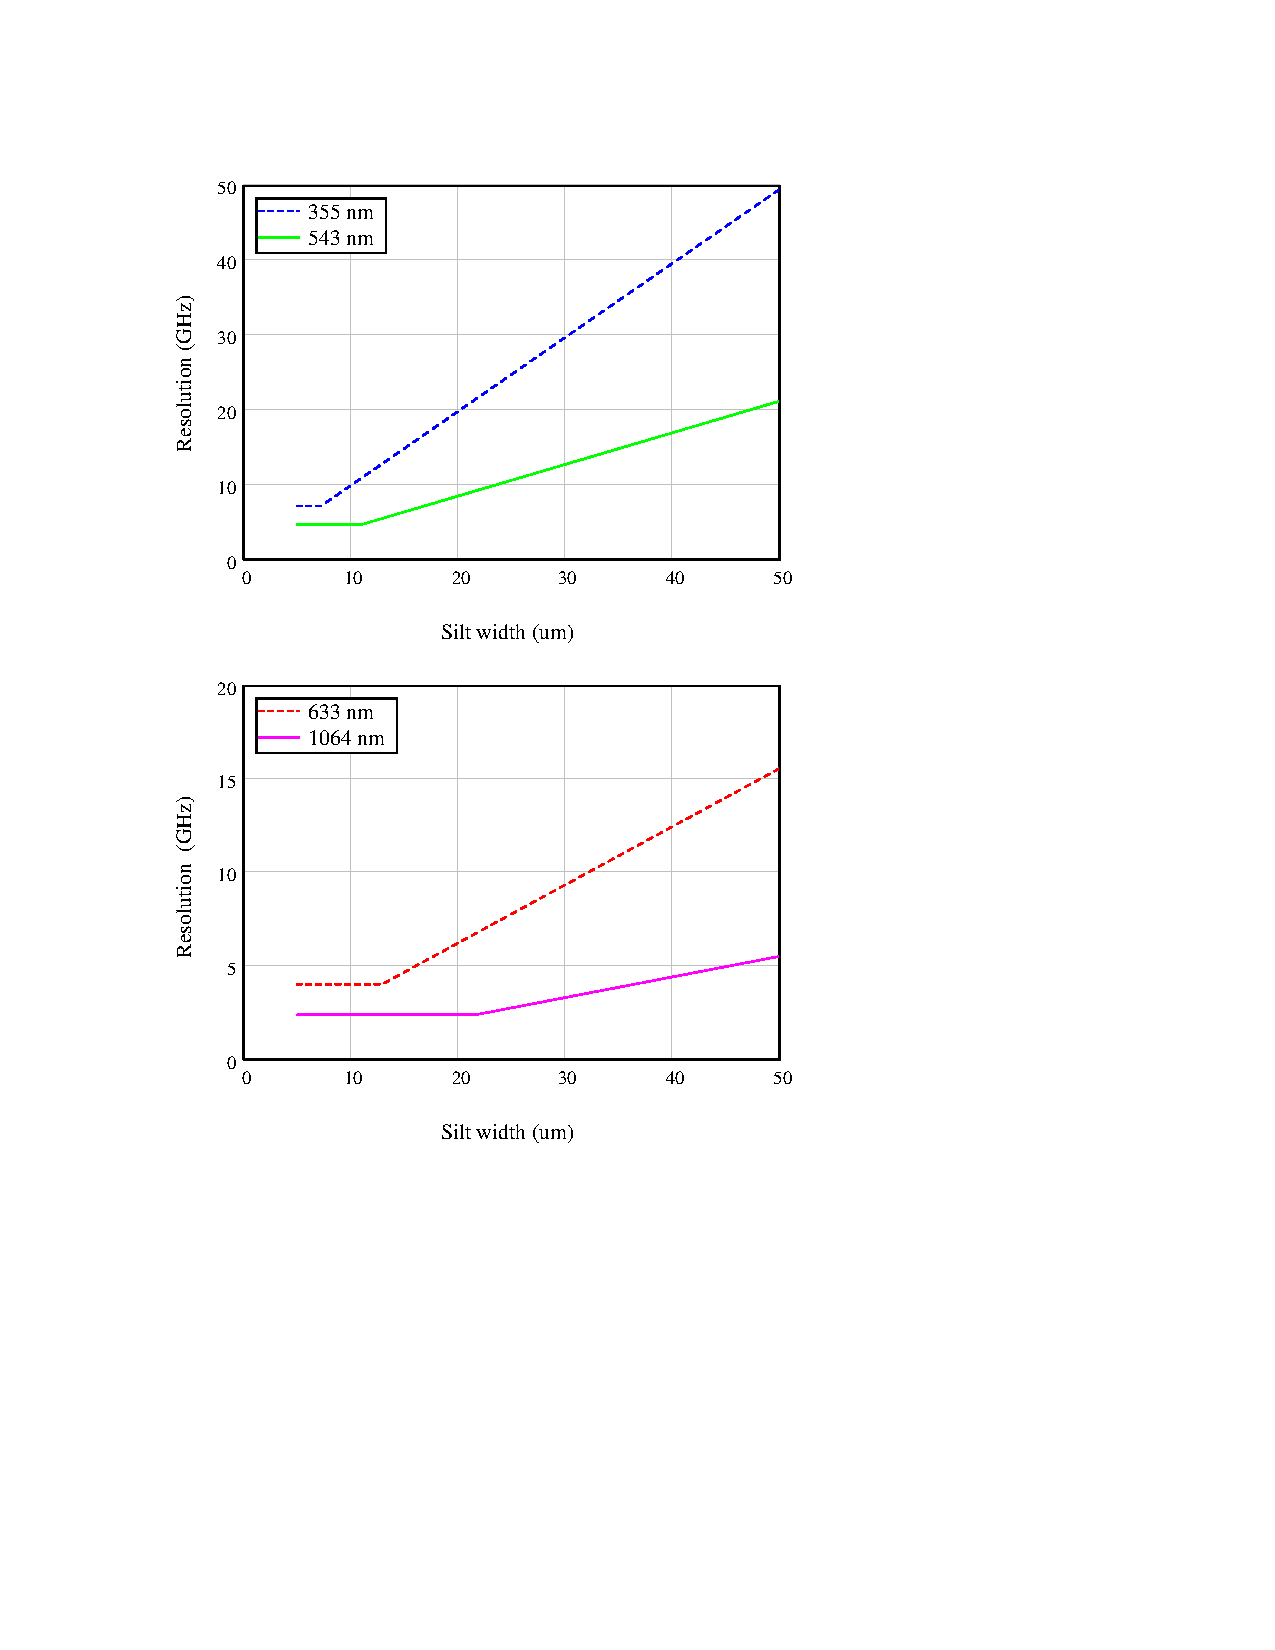
\includegraphics[bb=-30 250 489 700]
{near_GHz/near_GHz.pdf}
}
\caption{Ideal 1 m monochromator resolution (GHz)}
\label{near_GHz}
\end{figure}
%----------------------------------------------------------------------------

%----------------------------------------------------------------------------
%----------------------------------------------------------------------------
%----------------------------------------------------------------------------
%bb defines the bounding box for the pdf
%viewport defines the area of the pdf used
%in sidewaysfigure the last entry in bb moves the caption toward/away the pic
%in sidewaysfigure the second entry in bb moves the pic toward/away the caption
%----------------------------------------------------------------------------
\begin{figure}
\scalebox{0.8}[0.8]{
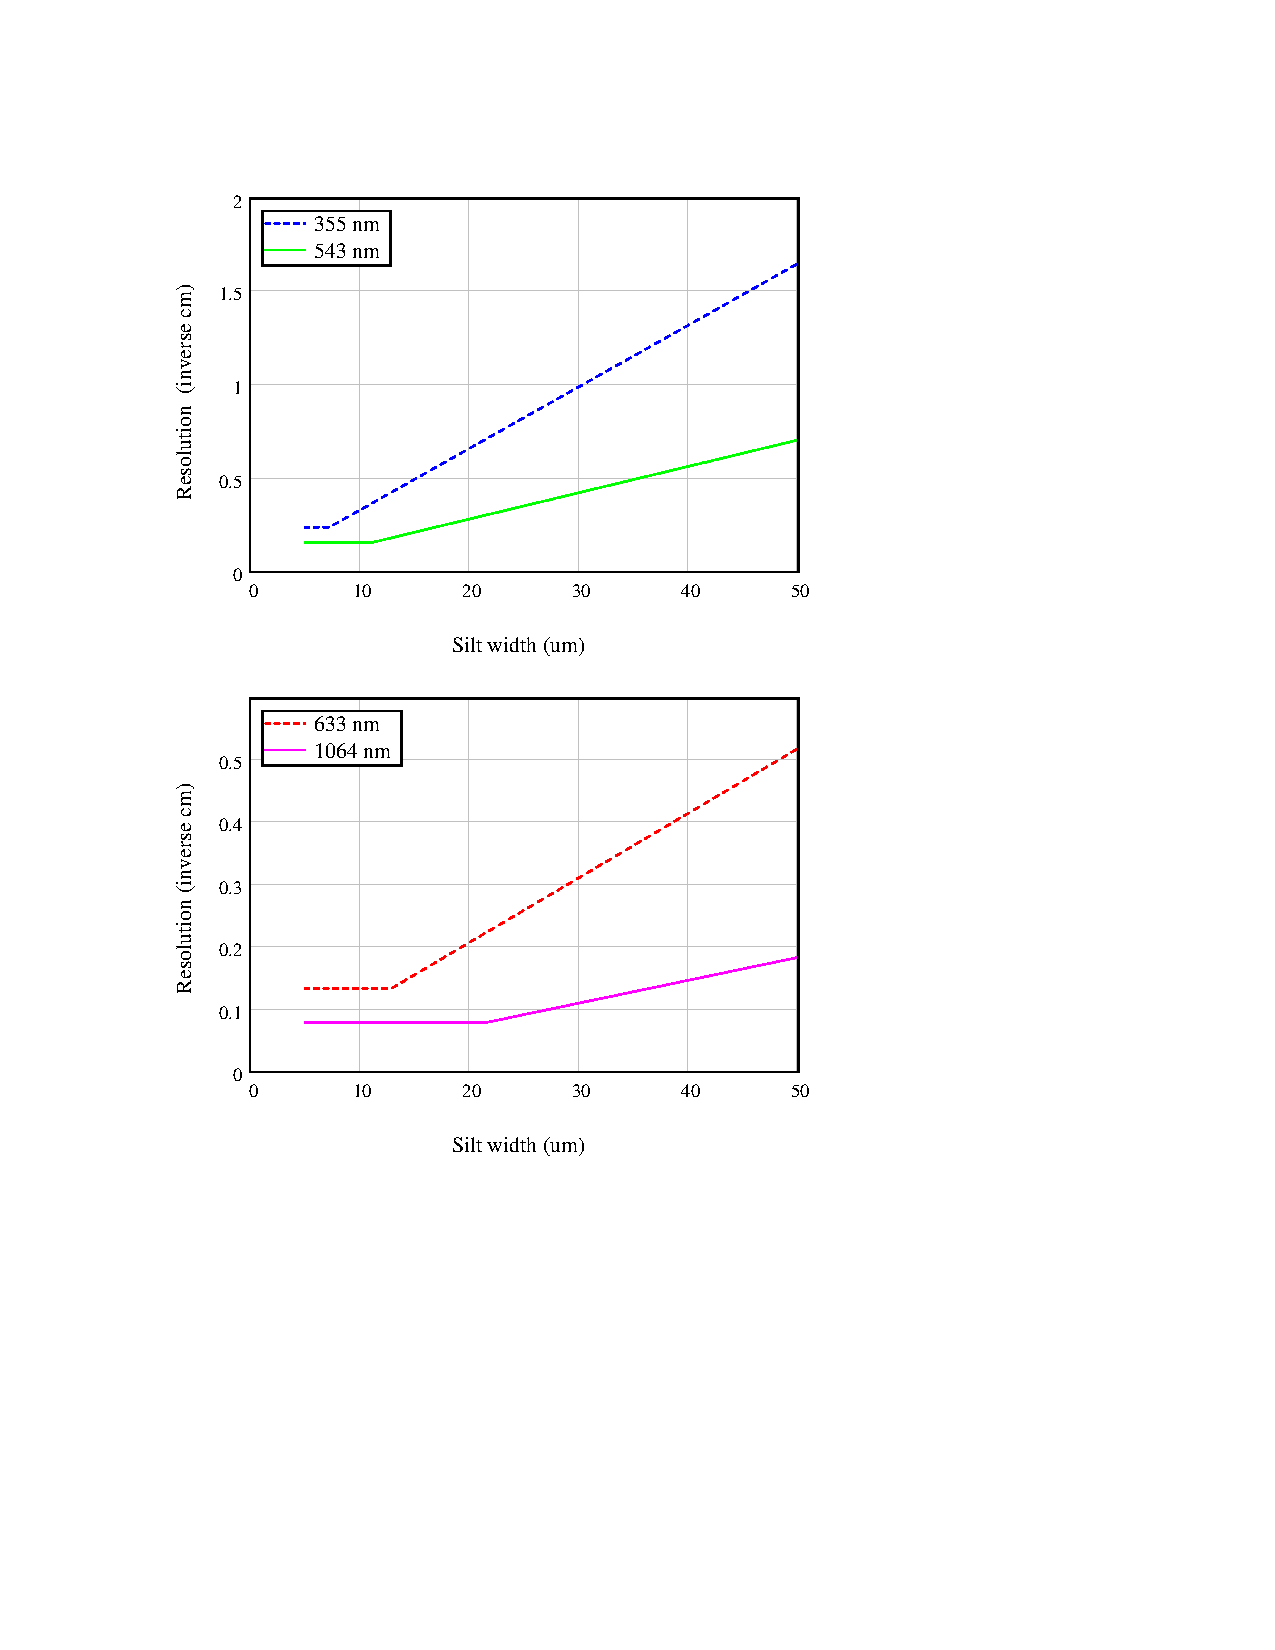
\includegraphics[bb=-30 245 489 600]
{near_cm/near_cm.pdf}
}
\caption{Ideal 1 m monochromator resolution (inverse cm)}
\label{near_cm}
\end{figure}
%----------------------------------------------------------------------------

%----------------------------------------------------------------------------
%----------------------------------------------------------------------------
%----------------------------------------------------------------------------
%bb defines the bounding box for the pdf
%viewport defines the area of the pdf used
%in sidewaysfigure the last entry in bb moves the caption toward/away the pic
%in sidewaysfigure the second entry in bb moves the pic toward/away the caption
%----------------------------------------------------------------------------
\begin{figure}
\scalebox{0.8}[0.8]{
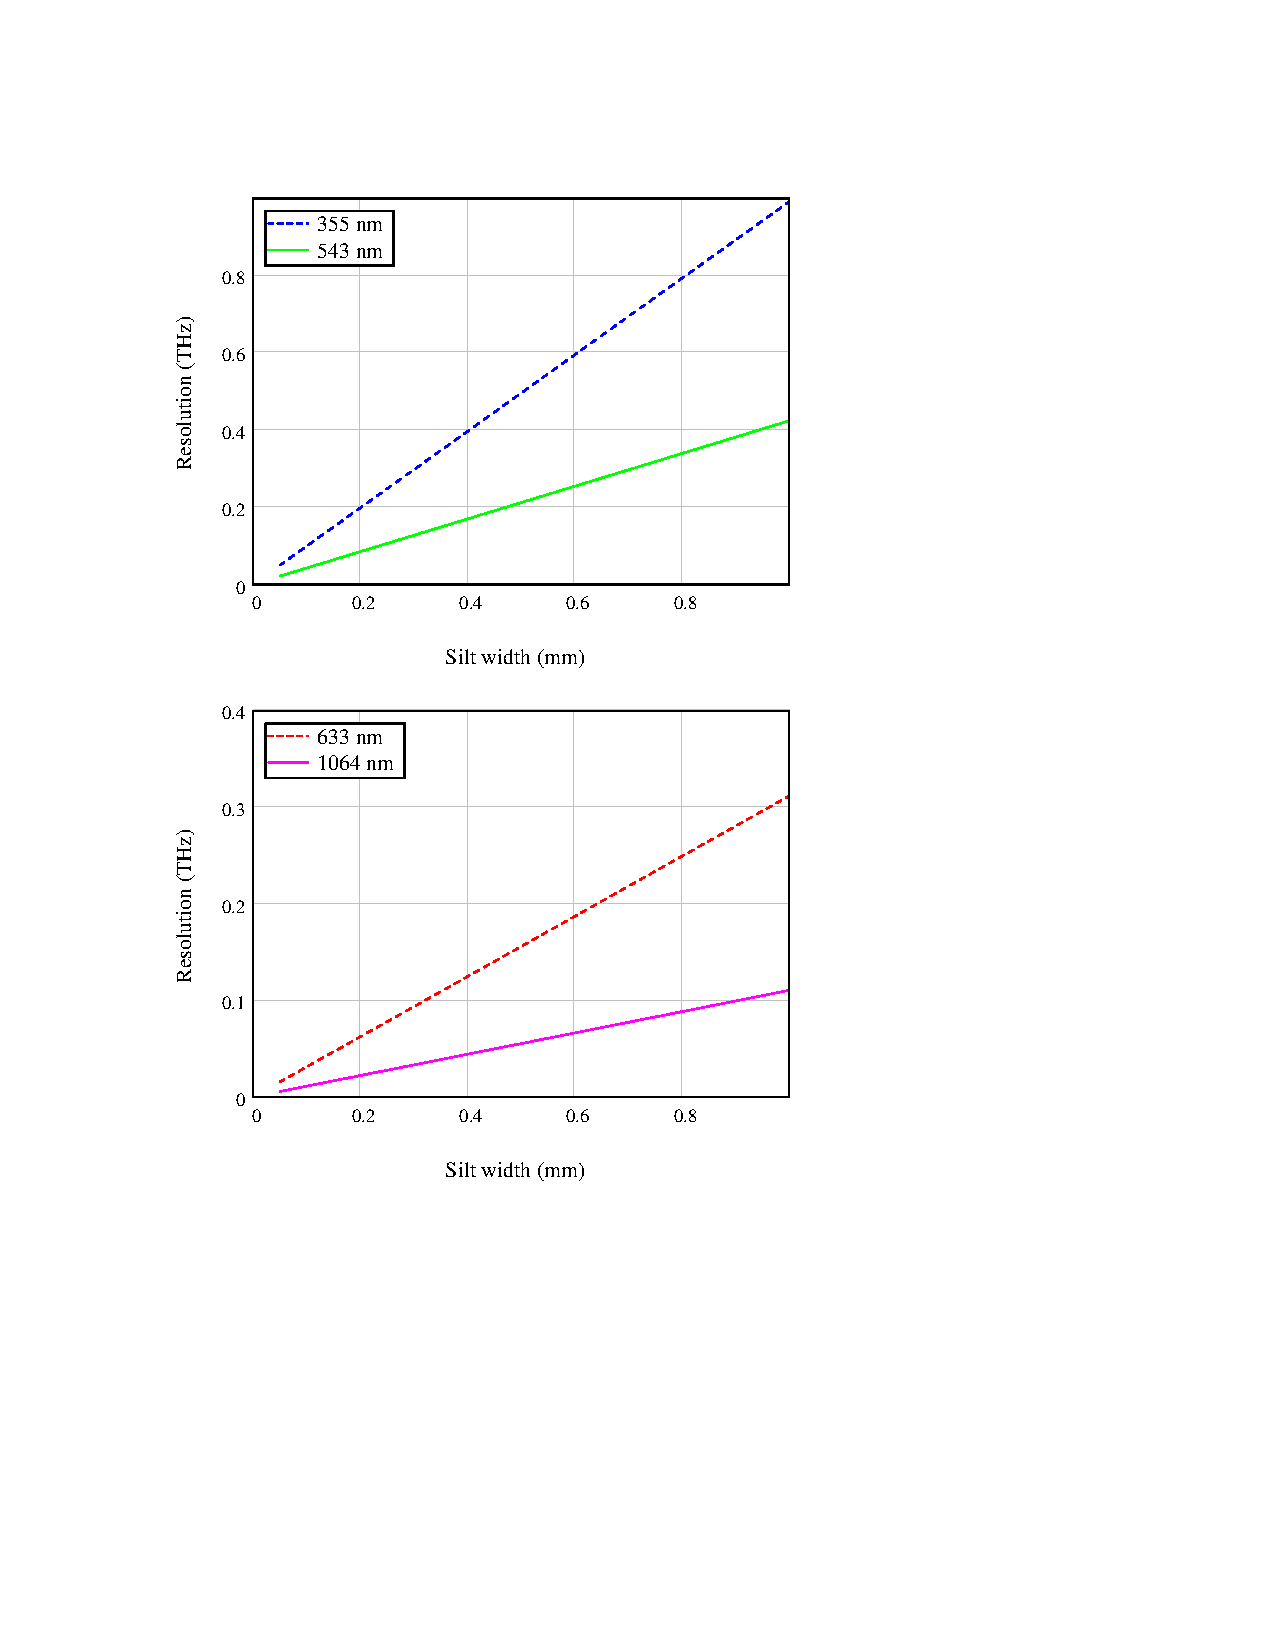
\includegraphics[bb=-30 230 489 700]
{far_THz/far_THz.pdf}
}
\caption{Ideal 1 m monochromator resolution (THz) for large slit widths}
\label{far_THz}
\end{figure}
%----------------------------------------------------------------------------

%----------------------------------------------------------------------------
%----------------------------------------------------------------------------
%----------------------------------------------------------------------------
%bb defines the bounding box for the pdf
%viewport defines the area of the pdf used
%in sidewaysfigure the last entry in bb moves the caption toward/away the pic
%in sidewaysfigure the second entry in bb moves the pic toward/away the caption
%----------------------------------------------------------------------------
\begin{figure}
\scalebox{0.8}[0.8]{
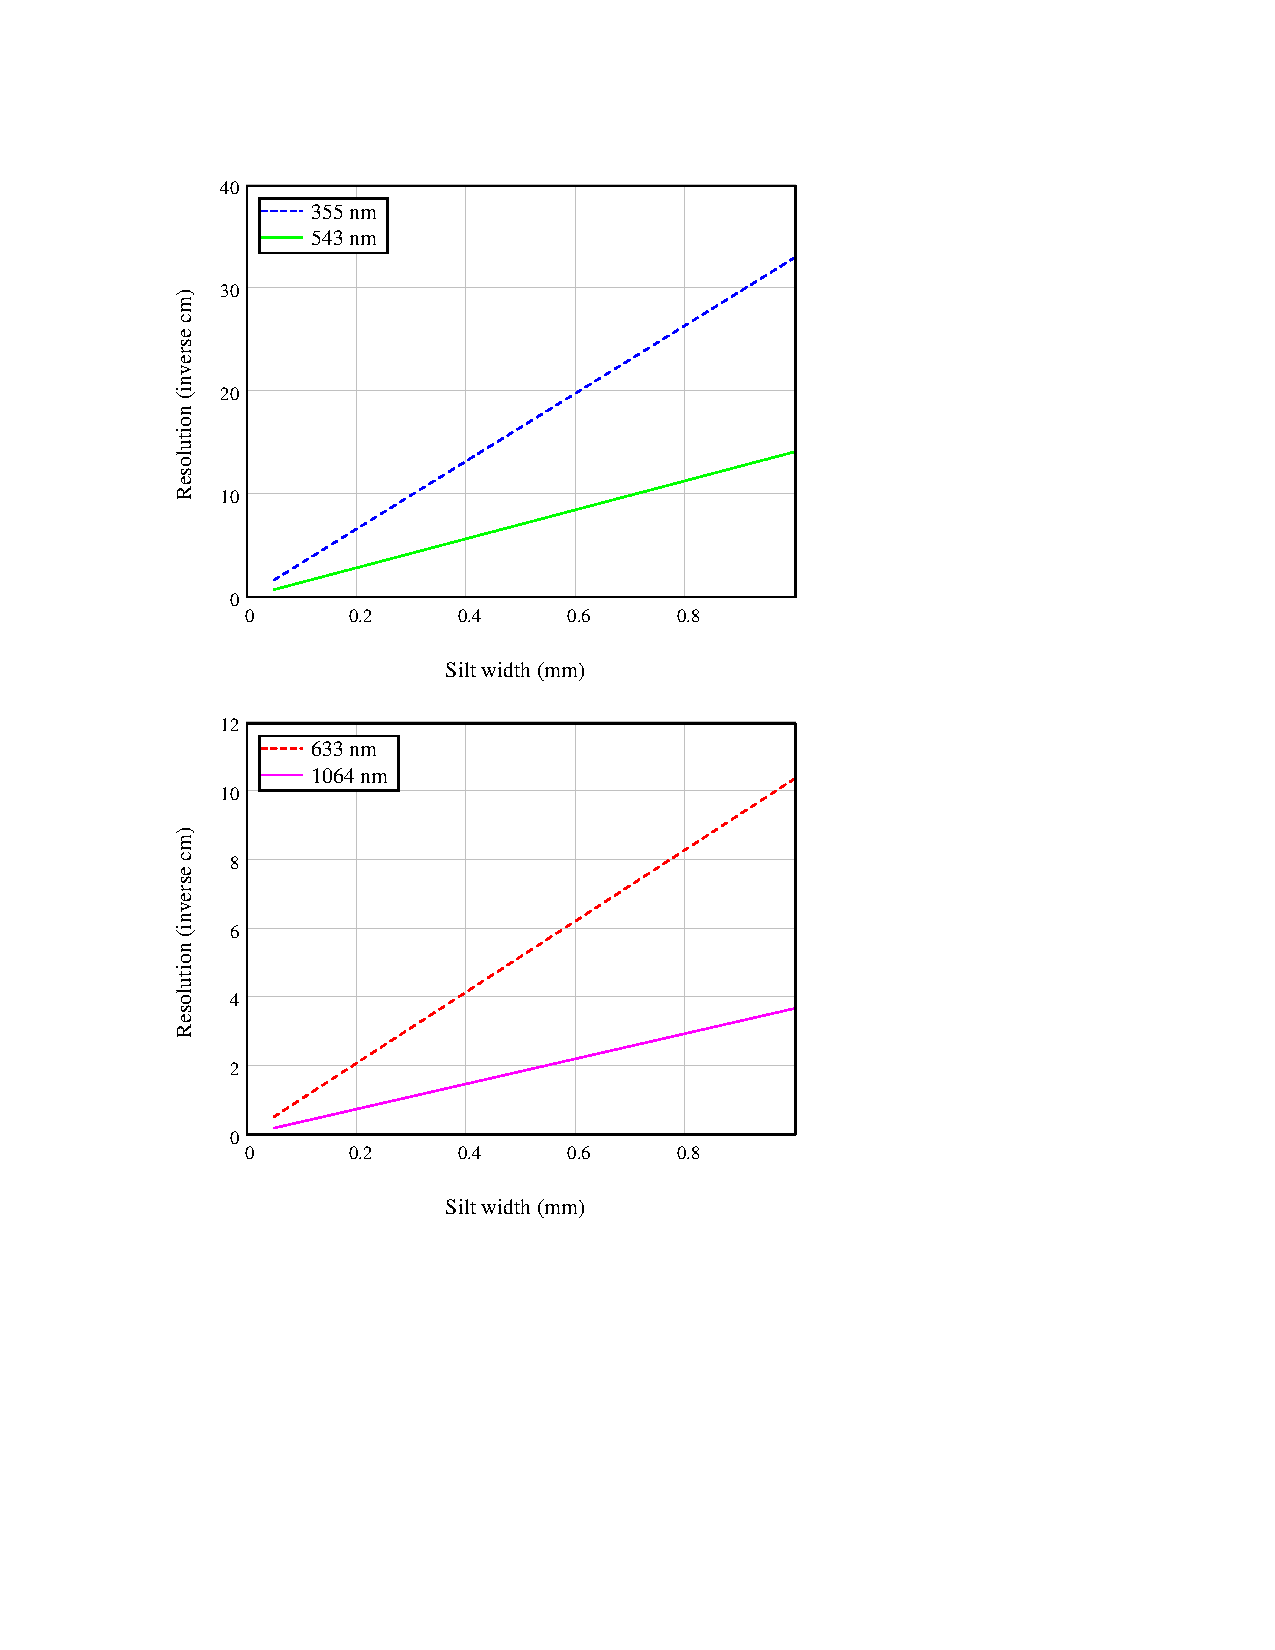
\includegraphics[bb=-30 212 489 700]
{far_cm/far_cm.pdf}
}
\caption{Ideal 1 m monochromator resolution (inverse cm) for large slit widths}
\label{far_cm}
\end{figure}
%----------------------------------------------------------------------------

%----------------------------------------------------------------------------
%----------------------------------------------------------------------------
%----------------------------------------------------------------------------
%bb defines the bounding box for the pdf
%viewport defines the area of the pdf used
%in sidewaysfigure the last entry in bb moves the caption toward/away the pic
%in sidewaysfigure the second entry in bb moves the pic toward/away the caption
%----------------------------------------------------------------------------
\begin{figure}
\scalebox{0.8}[0.8]{
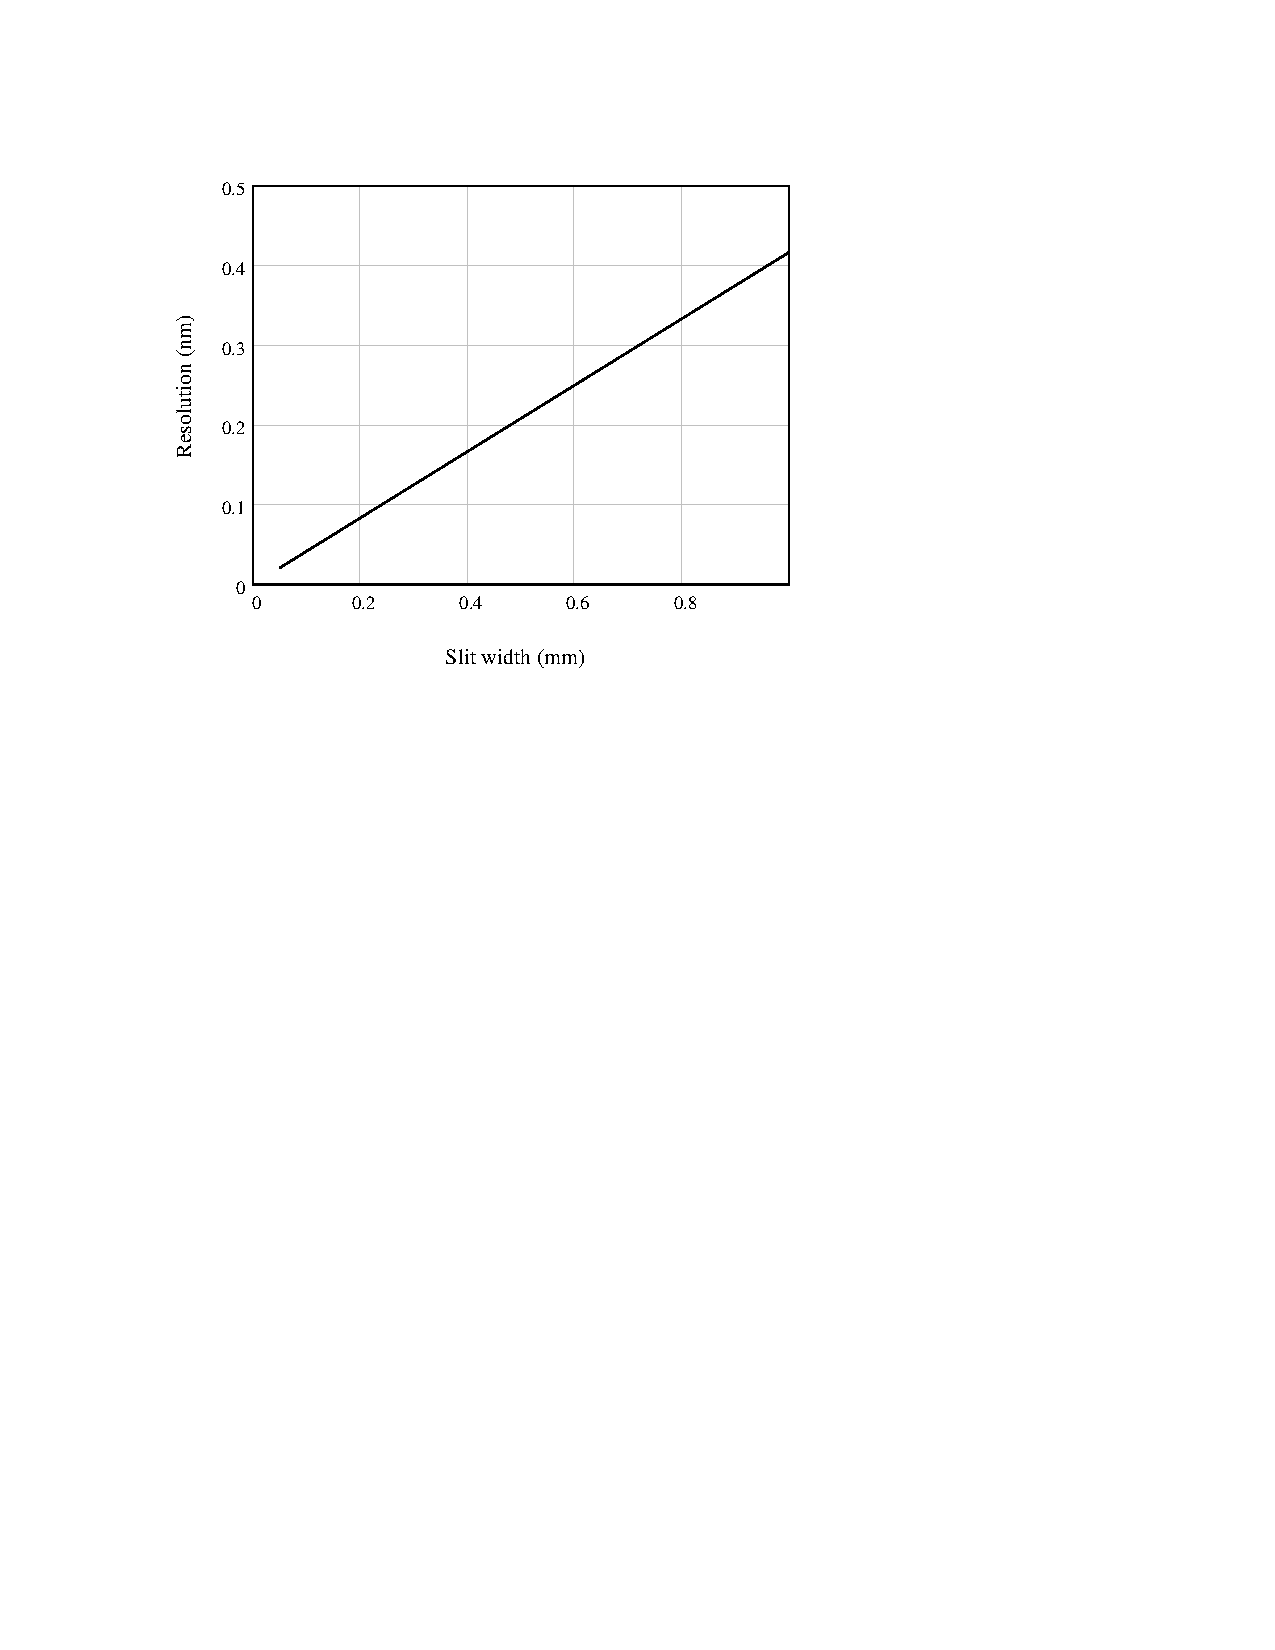
\includegraphics[bb=-30 478 489 700]
{far_nm/far_nm.pdf}
}
\caption[Ideal 1 m monochromator resolution (nm) for large slit widths]{Ideal 1 m monochromator resolution (nm) for large slit widths - Equations \ref{Rayleigh} and \ref{resolvance} imply $\Delta\lambda = a/(2mL\rho)$; here the resolution ($\Delta\lambda$) is ploted for $m=1$, $L=1$ m, and $\rho=1200$ lines per mm.}
\label{far_nm}
\end{figure}
%----------------------------------------------------------------------------

%----------------------------------------------------------------------------
%----------------------------------------------------------------------------
%----------------------------------------------------------------------------
%----------------------------------------------------------------------------

%----------------------------------------------------------------------------
\subsection{Velocity distribution}
%----------------------------------------------------------------------------
%----------------------------------------------------------------------------
%----------------------------------------------------------------------------
The distribution of molecular speeds in a gas is governed by Maxwell-Boltzmann statistics. This distribution impacts this study through the equation of motion (Equation \ref{final eom}) as a Doppler shift and through the ``geometric'' effects associated with linear molecular motion in the target region. The Doppler shift is proportional to the projection of the molecular velocity vector onto the laser beam wave front normal; the effects of the Doppler shift are described in Section \ref{doppler section}. The ``geometric'' effects are the temporal modulation of the excitation the molecule experiences by either leaving the excitation region before the pulse ends or entering the excitation region after the pulse has already started (or both). Additionally, the point in time at which the molecule emits its fluorescence photon may occur after the molecule leaves the region to which the receiver is sensitive.

The Maxwell-Boltzmann probability density function for molecular speeds is given by \cite{Serway:1990a}
%----------------------------------------------------------------------------
\begin{equation}
\rho(|v|)
=
\sqrt{\frac{2}{\pi}}
\left(\frac{m}{kT}\right)^{\frac{3}{2}}
v^2
\exp{\left(
-\frac{m v^2}{2 k T}
\right)}
\end{equation}
%----------------------------------------------------------------------------
where $k$ is the Boltzmann constant, T is the temperature (in K), $m$ is the molecular mass, and $v^2$ is the square of the molecular speed. See Figure \ref{Boltzmann-Maxwell} for a plot of this distribution.
%----------------------------------------------------------------------------
%----------------------------------------------------------------------------
%bb defines the bounding box for the pdf
%viewport defines the area of the pdf used
%in sidewaysfigure the last entry in bb moves the caption toward/away the pic
%in sidewaysfigure the second entry in bb moves the pic toward/away the caption
%----------------------------------------------------------------------------
\begin{figure}
\scalebox{0.8}[0.8]{
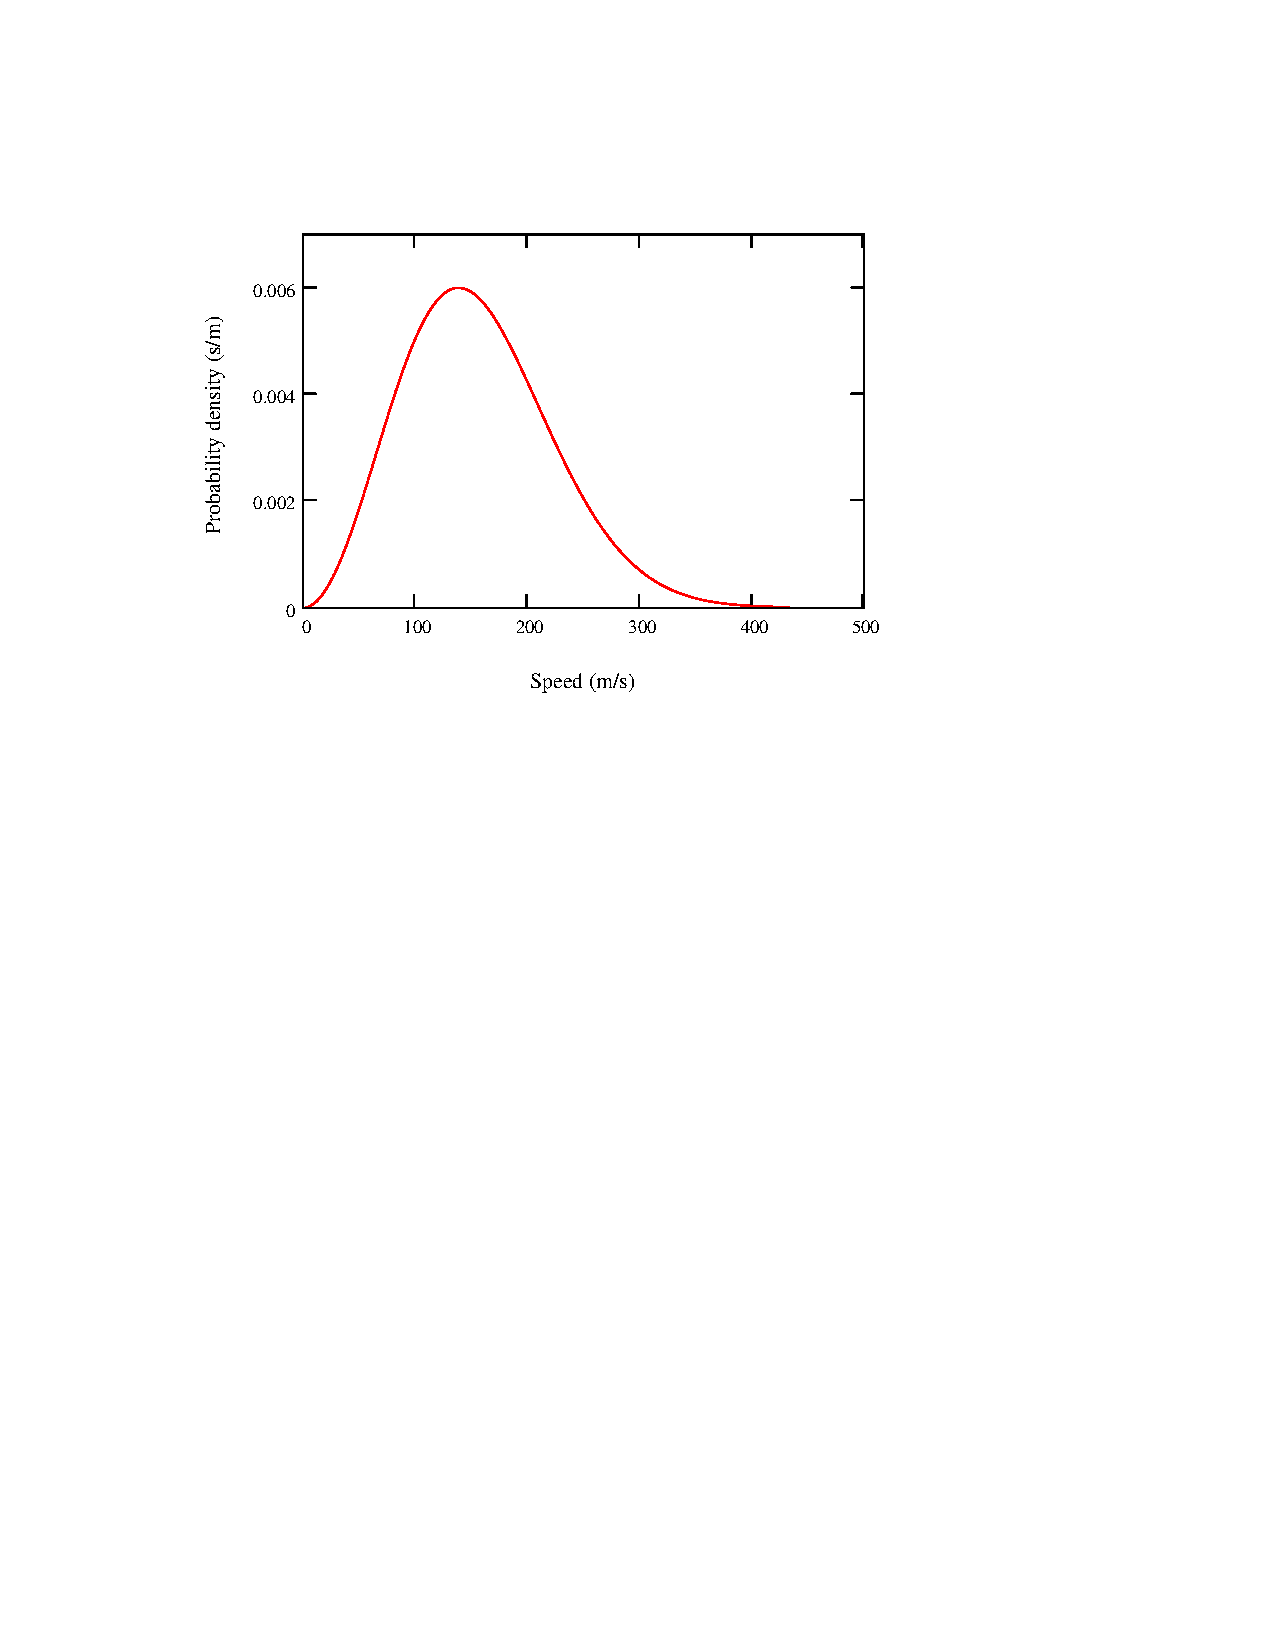
\includegraphics[bb=0 470 489 675]
{Boltzmann-Maxwell/Boltzmann-Maxwell.pdf}
}
\caption[Boltzmann-Maxwell distribution for molecular iodine]{Boltzmann--Maxwell distribution for molecular iodine. For this plot and associated simulations, $T=293$ K, $m = 2 \cross 127$ u (u $= 1.6605402\cross10^{-27}$ kg). The root mean square speed is 167 m/s, the average speed is 156 m/s, and the most probable speed is 139 m/s.}
\label{Boltzmann-Maxwell}
\end{figure}
%----------------------------------------------------------------------------

%----------------------------------------------------------------------------
%----------------------------------------------------------------------------
%----------------------------------------------------------------------------

%----------------------------------------------------------------------------
\subsection{Side view geometry}
%----------------------------------------------------------------------------
%bb defines the bounding box for the pdf
%viewport defines the area of the pdf used
%in sidewaysfigure the last entry in bb moves the caption toward/away the pic
%in sidewaysfigure the second entry in bb moves the pic toward/away the caption
%----------------------------------------------------------------------------
\begin{figure}
\scalebox{0.7}[0.7]{
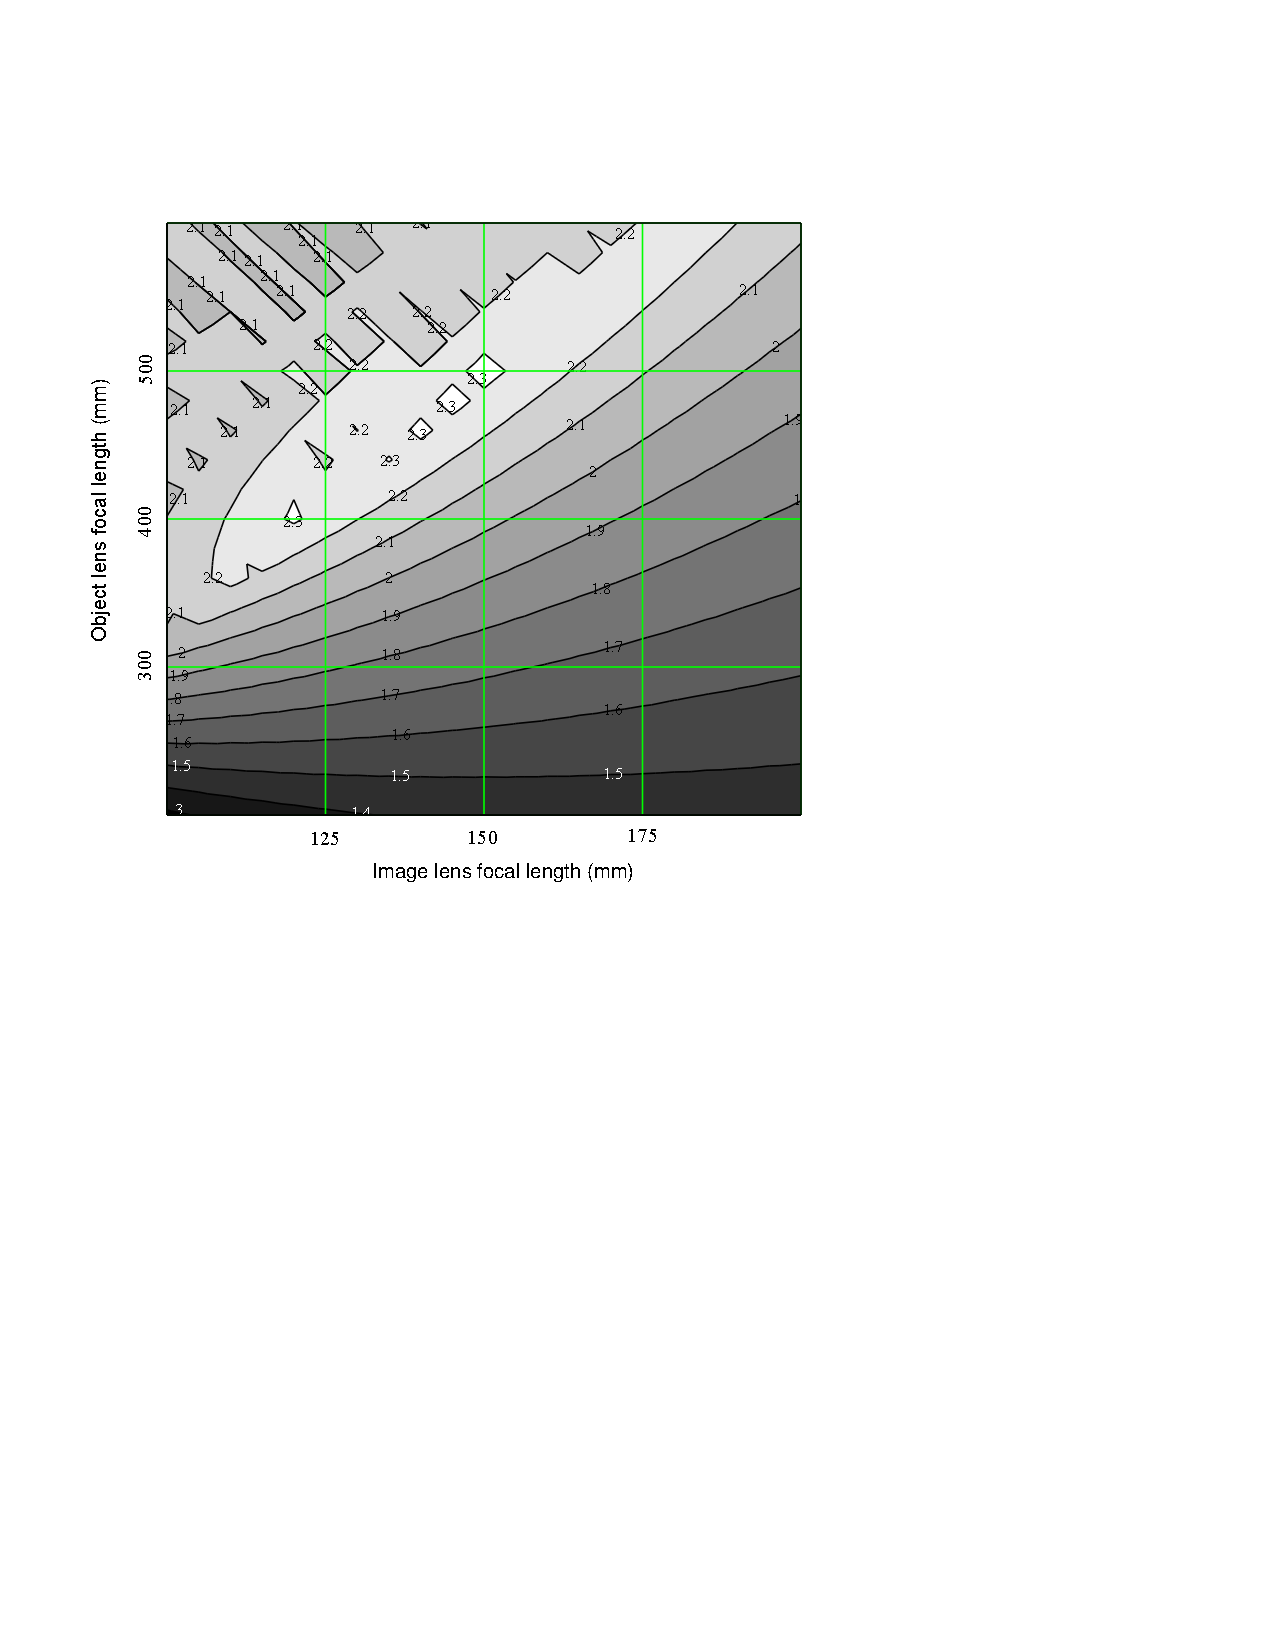
\includegraphics[bb=-60 360 489 725]
{side_view/side_view.pdf}
}
\caption[Side--view lens optimization surface]{Side--view lens optimization surface. For this calculation the beam waist diameter is 1 mm, the wavelength is 0.63 $\mu$m, the slitwidth is 300 $\mu$m, the slit height is 0.5 cm, and the monochromator acceptance angle is 52 mrad. The object lens is placed one focal length from the sample, while the image lens is placed one focal length from the monochromator input. The units for the contour in the plot are $10^{-12}$ m$^3$ (scaled volume). Thus if the target was air (near $10^{25}$ molecules per cubic meter) we would expect this system to be sensitive to $10^{13}$ atmospheric molecules (assuming all molecules decay optically in an isotropic fashion).}
\label{side_view}
\end{figure}
%----------------------------------------------------------------------------

%----------------------------------------------------------------------------
\subsection{Backscatter geometry}
\label{backscatter section}
%----------------------------------------------------------------------------
Consider an optical setup where a laser beam line is merged with receiver beam line. The merge could be facilitated through the use of a dichroic beam splitter: reflecting the wavelength associated with the laser while transmitting the broad spectrum associated with the fluorescence radiation. By allowing some of the laser focusing optics to double as the receiver optics gives rise to unique geometries where the receiver and laser source are localized and their beam lines are extended to some remote target region (a LIDAR application). See Figure \ref{backscatter_figure} for a beam line diagram.
%----------------------------------------------------------------------------
%----------------------------------------------------------------------------
%bb defines the bounding box for the pdf
%viewport defines the area of the pdf used
%in sidewaysfigure the last entry in bb moves the caption toward/away the pic
%in sidewaysfigure the second entry in bb moves the pic toward/away the caption
%----------------------------------------------------------------------------
\begin{figure}
\scalebox{0.6}[0.6]{
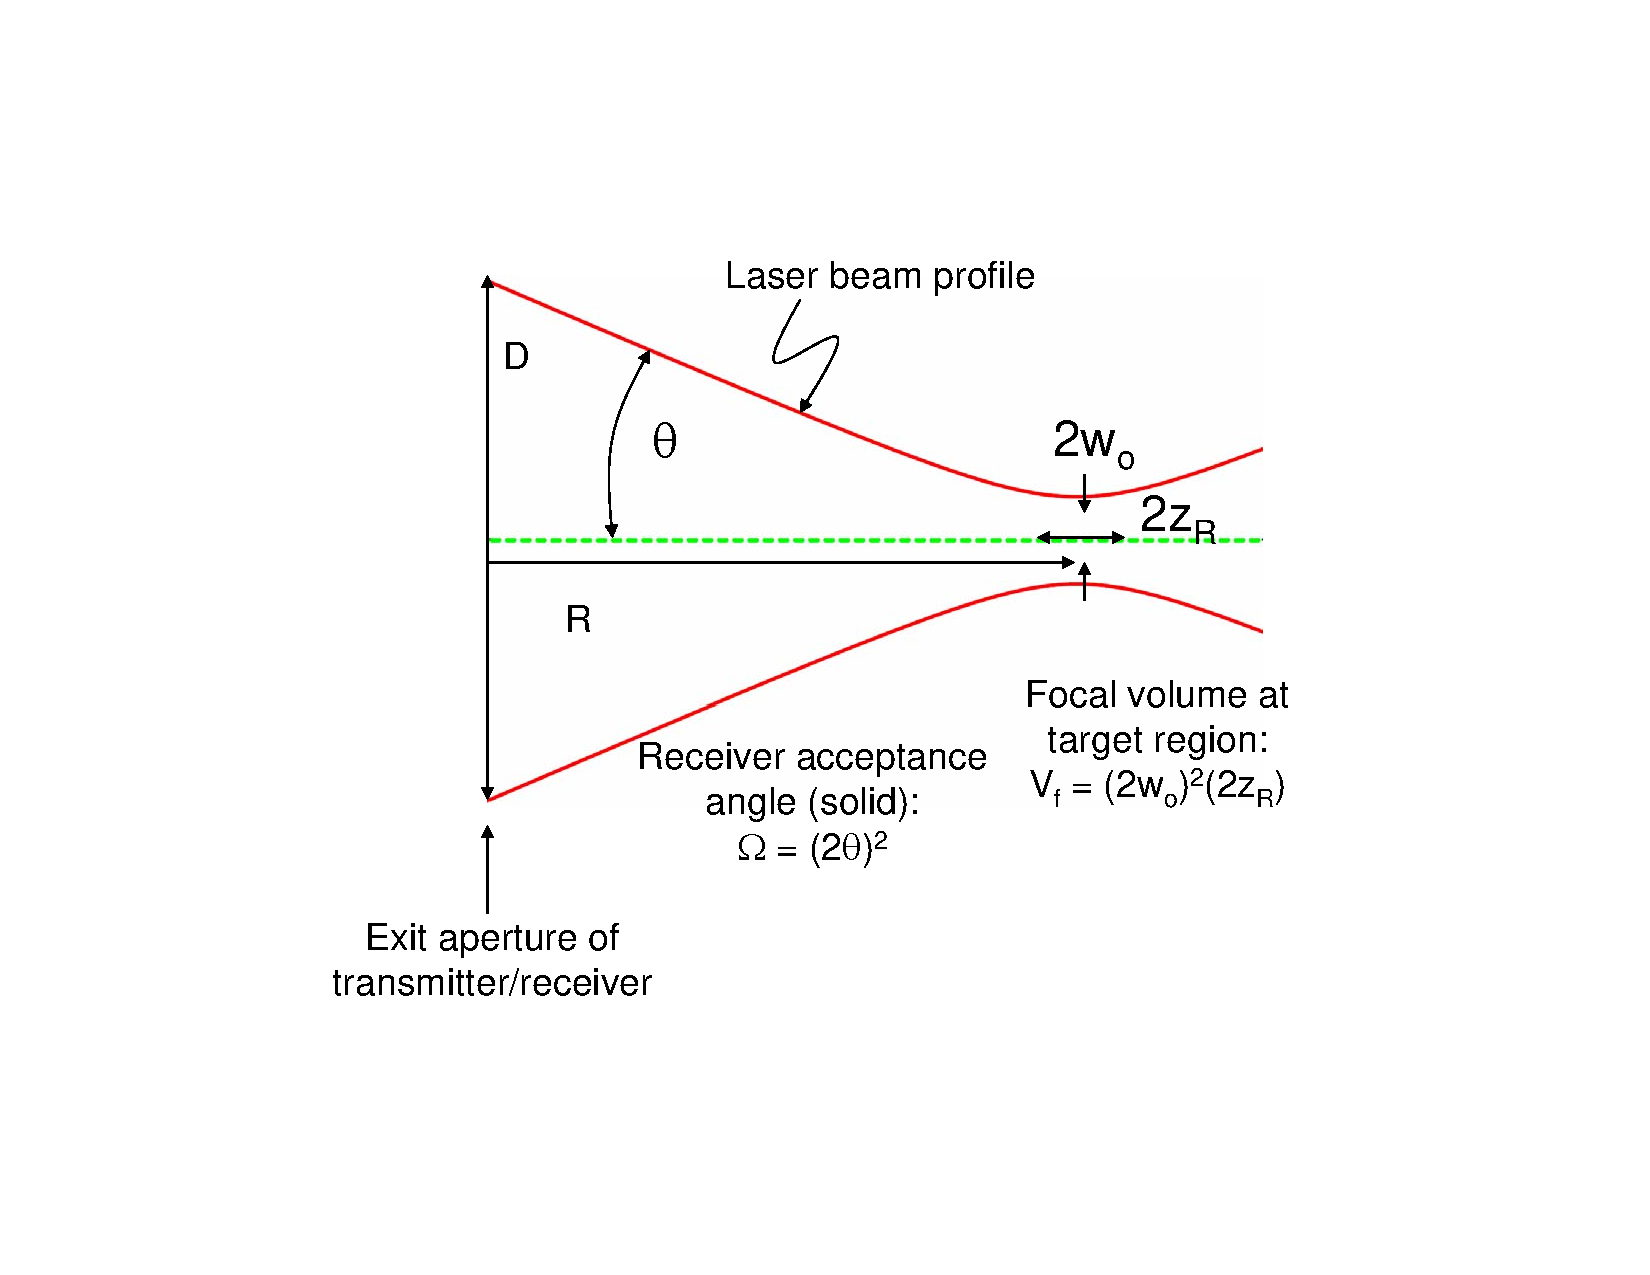
\includegraphics[bb=35 125 489 480]
{backscatter_figure/backscatter_figure.pdf}
}
\caption[Backscatter geometry]{Backscatter geometry. After leaving the exit aperture of diameter D, a laser beam is brought to a focus a distance R from the aperture. The dimensions of the focal volume and the far-field divergence ($\theta$) depend only on D, R, and the laser wavelength $\lambda$.}
\label{backscatter_figure}
\end{figure}
%----------------------------------------------------------------------------

%----------------------------------------------------------------------------

The probability of photon detection is proportional to
%----------------------------------------------------------------------------
\begin{equation}
ABCD
\int\int
\rho(\vec{r})
P(\vec{r},t)
\Phi(\vec{r},\hat{c})
d\vec{r}
d\Omega
\label{total_prob}
\end{equation}
%----------------------------------------------------------------------------
where $A$ is the fraction of target molecules which couple to the laser radiation, $B$ represents atmospheric attenuation effects like Mie scattering, absorption, etc., $C$ represents the fraction of excited molecules that decay optically within the bandwidth of the detector, $D$ represents the fraction of optically decaying molecules which emit a photon before collisional effects force non-optical decay (see discussion at the end of Section \ref{side}), $\rho(\vec{r})$ is the density distribution of the target molecules, $P(\vec{r},t)$ is the molecular inversion probability (this is a function of the fluence at position $\vec{r}$ and at time $t$), $\Phi(\vec{r},\hat{c})$ is the phase space factor (a function of position as well as the direction of travel of the emitted photon $\hat{c}$). In the following analysis some approximations are made to estimate this integral. First we ignore $A$, $B$, $C$, and $D$, thus we simply calculate the photon capture probability assuming all molecules optically decay isotropically. The density is assumed uniform, $\Phi$ is simply taken to limit the integration volume to the focal volume and introduce a factor equal to the solid angle fraction available to the detector from the target region, and $P$ is assumed to be equal to unity.
%----------------------------------------------------------------------------
%----------------------------------------------------------------------------
%bb defines the bounding box for the pdf
%viewport defines the area of the pdf used
%in sidewaysfigure the last entry in bb moves the caption toward/away the pic
%in sidewaysfigure the second entry in bb moves the pic toward/away the caption
%----------------------------------------------------------------------------
\begin{figure}
\scalebox{0.8}[0.8]{
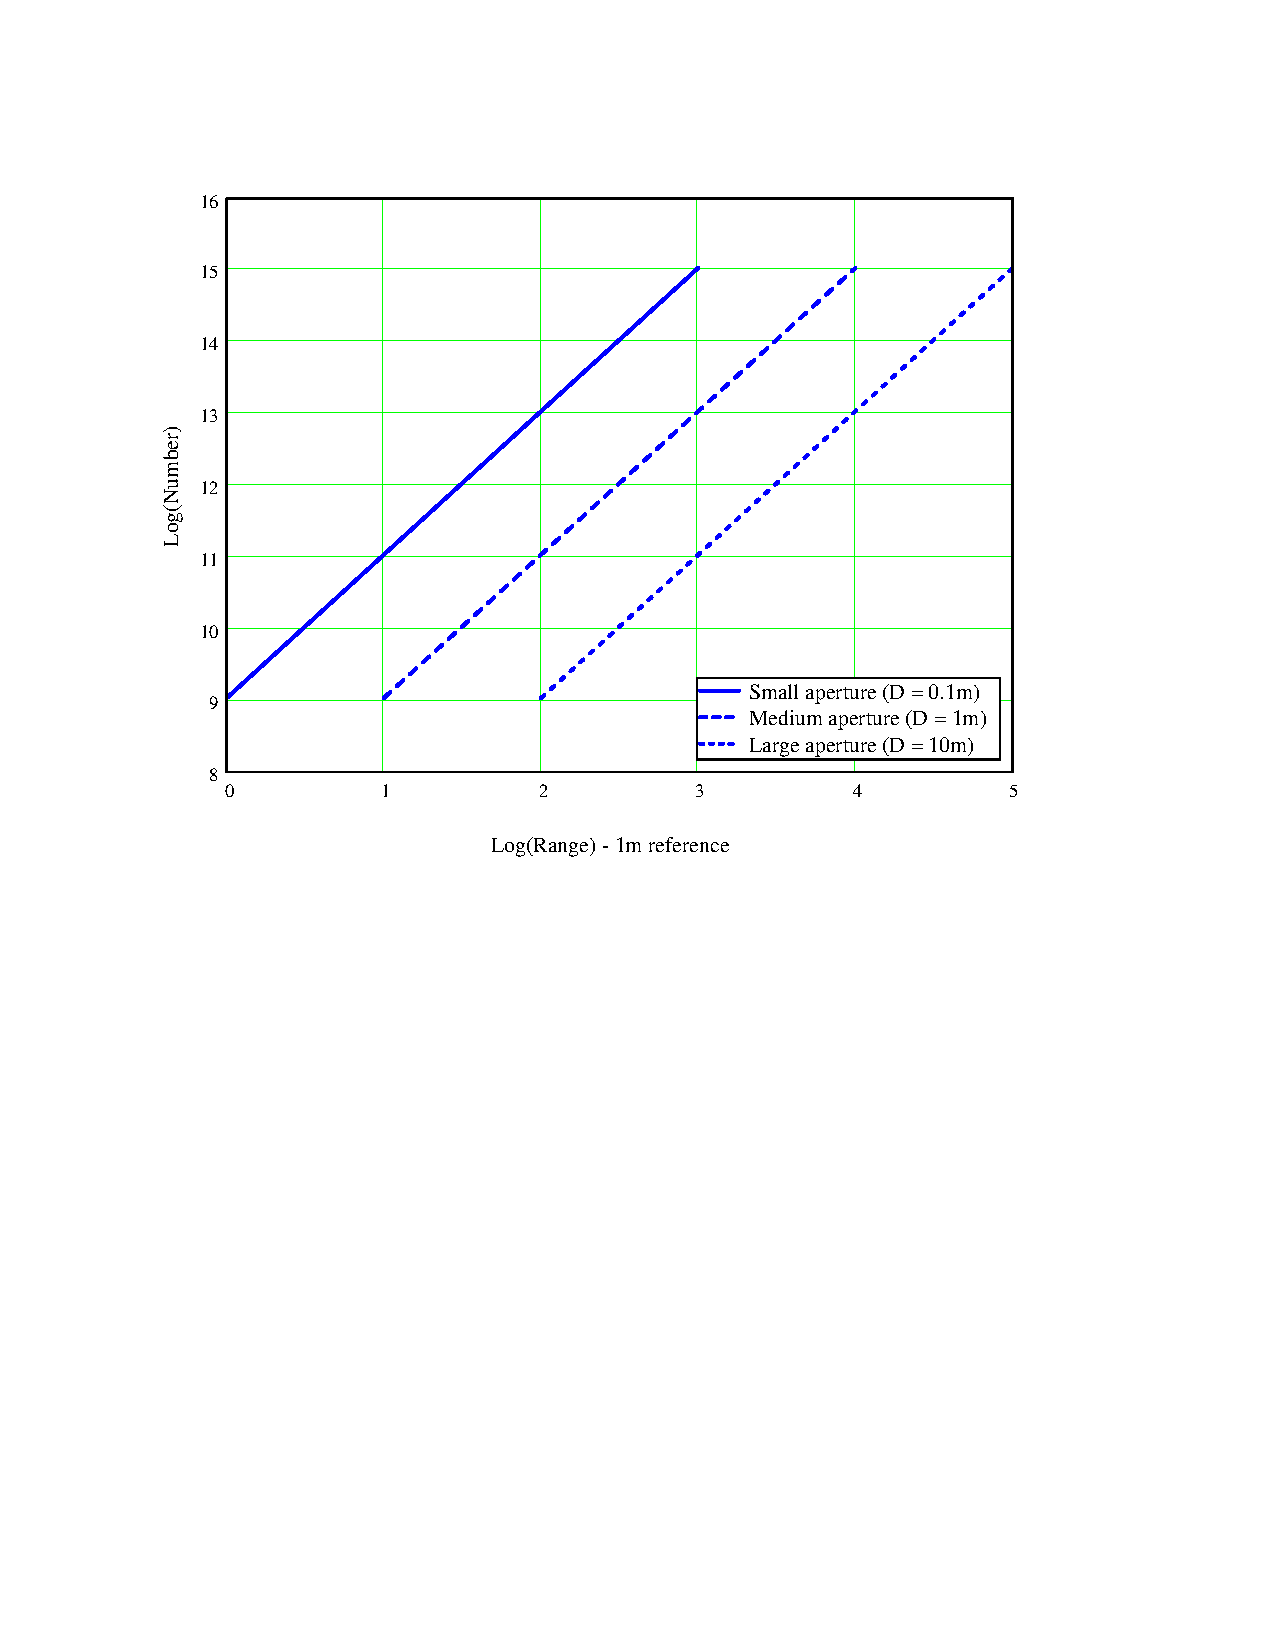
\includegraphics[bb=20 390 489 680]
{back_number/back_number.pdf}
}
\caption[Number of molecules emitting into reciever in a LIDAR application]{Number of molecules emitting into reciever acceptance area (ideal: $A=B=C=D\equiv1$ in Equation \ref{total_prob}). The ratio $R/D$ must be larger than unity to satisfy the approximations used to construct Equations \ref{energy_required} and \ref{v_eff}. Here we have used $\lambda=1$ $\mu$m, and a density of $10^{25}$ molecules per m$^3$. Thus, with an aperture of $D=1$ m and a focal length of 1 km, we expect the system to be sensitive to at most $10^{13}$ atmospheric molecules.}
\label{back_number}
\end{figure}
%----------------------------------------------------------------------------

%----------------------------------------------------------------------------

The output aperture, with diameter $D$, is taken as the origin and the target is at the focus of a Gaussian beam which is some distance, $R$, from the output aperture. The Gaussian beam emerges from the output aperture with a clear aperture compatible with a far-field ripple of less than 1\% \cite{Siegman:1986a}. The integration limits are taken as the boundaries of a rectangular volume centered at the focus: the extent of the region along the beam axis is taken as the Rayleigh range and the transverse dimensions are taken as the waist diameter. The solid angle fraction is taken as
%----------------------------------------------------------------------------
\begin{equation}
\frac{(2\theta)^2}{4\pi}
\end{equation}
%----------------------------------------------------------------------------
where $\theta$ is the far-field divergence \emph{half} angle of the Gaussian beam \cite{Siegman:1986a}. Using these ideas, one can arrive at the following expression for the scaled volume (the product of the volume and the solid angle fraction)
%----------------------------------------------------------------------------
\begin{equation}
\boxed{
V_{eff}
=
\frac{4.6^2}{2 \pi^2}
\lambda^3
\left(\frac{R}{D}\right)^2.
\label{v_eff}
}
\end{equation}
%----------------------------------------------------------------------------
The required pulse energy depends on the fluence (Equation \ref{required fluence}) and the focal spot diameter. The relationship is
%----------------------------------------------------------------------------
\begin{equation}
\boxed{
E
=
\frac{42.32}{\pi}
c \hbar^2 \epsilon_o
\frac{(\Delta\tau)^2}{M^2 t}
\lambda^2
\left(\frac{R}{D}\right)^2.
\label{energy_required}
}
\end{equation}
%----------------------------------------------------------------------------
See Figures \ref{back_number} and \ref{back_energy} for plots of these functions for various aperture sizes.

%----------------------------------------------------------------------------
%----------------------------------------------------------------------------
%bb defines the bounding box for the pdf
%viewport defines the area of the pdf used
%in sidewaysfigure the last entry in bb moves the caption toward/away the pic
%in sidewaysfigure the second entry in bb moves the pic toward/away the caption
%----------------------------------------------------------------------------
\begin{figure}
\scalebox{0.8}[0.8]{
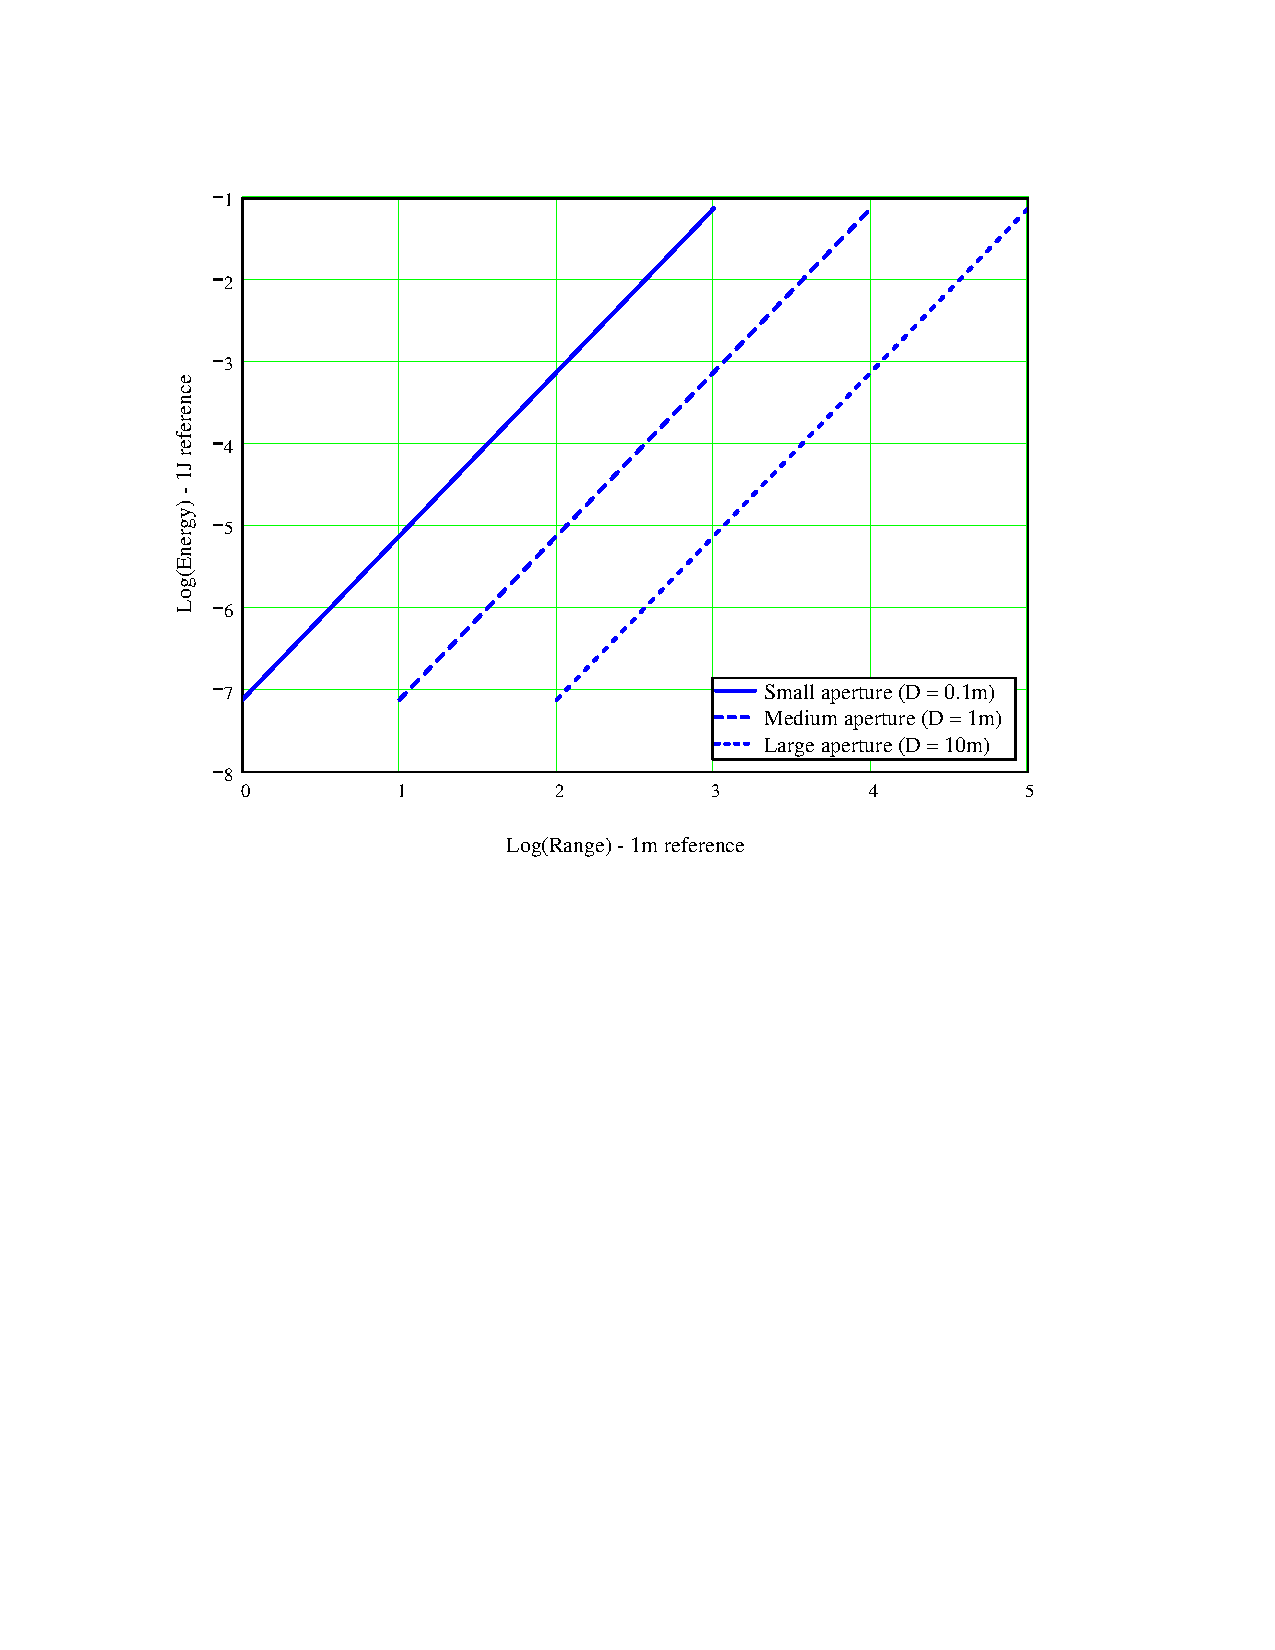
\includegraphics[bb=20 390 489 700]
{back_energy/back_energy.pdf}
}
\caption[Required pulse energy to invert target molecules]{Required pulse energy to invert target molecules. Here we have used the dipole matrix element approximated in Section \ref{iodine} ($M=3.6\cross10^{-32}$ Cm), tophat pulse duration $t=1$ ns, $\lambda=1$ $\mu$m, and $\Delta \tau=\pi/2$ in Equation \ref{energy_required}.}
\label{back_energy}
\end{figure}
%----------------------------------------------------------------------------

%----------------------------------------------------------------------------

The key features of these equations illustrate the potential sensitivity and limitations of LIDAR geometries when one is concerned with LIF type experiments. The effective sensitive volume, Equation \ref{v_eff}, \emph{increases} as the square range, $R$. The obvious drawback is seen in Equation \ref{energy_required} where the required energy also increases with the square of the range. Indeed the ratio
%----------------------------------------------------------------------------
\begin{equation}
\frac{V}{E}
=
\frac{1}{4 \pi c \hbar^2 \epsilon_o}
\frac{M^2 t}{(\Delta\tau)^2}
\lambda
\label{LIDAR eff}
\end{equation}
%----------------------------------------------------------------------------
should be maximized for the most efficient application. $\lambda$ has a natural upper limit set by atmospheric transmission: optical wavelengths greater than 10 um are heavily attenuated. Collisional damping at STP forces $t$ to be less than 1 ns. $\Delta\tau$ is $\pi/2$ for Rabi oscillation population inversion; however, some coherent process require the quantity to increase by an order of magnitude or more (see Chapter \ref{computer chapter}). Most molecules have matrix elements, $M$, around one D ($\mbox{D}=10^{-18}\mbox{ esu}$ and $1\mbox{ Cm}=2.99792458\cross10^{9}\mbox{ esu}$).
%----------------------------------------------------------------------------
%----------------------------------------------------------------------------

%----------------------------------------------------------------------------
%----------------------------------------------------------------------------
\section{Conclusion}
%----------------------------------------------------------------------------
%------------------------------Broad objectives------------------------------
%----------------------------------------------------------------------------
This chapter chronicles the stages of laboratory development undergone over the past few years. The main measurements at each stage were used as a guide to develop the equipment and techniques required for demonstration of molecular control in LIDAR systems.
%----------------------------------------------------------------------------
%----------------------------------So what?----------------------------------
%----------------------------------------------------------------------------

As each stage was completed various components of the apparatus were either designed and assembled or evolved to the next generation. After the installation of the PMT at its output the monochromator served each experiment well until the recent aromatic compound measurements. The Hg pulser and Pockles cell system went through various stages of development starting with the initial tests of the Hg pulser on LED's to the integration of the system with the YAG pumped dye laser system during the fluorescence line decay measurements. The software model was tested at each stage from the familiar non-resonant HeNe LIF to pulsed resonant dye LIF. The data acquisition system was built for the first dye laser experiments and has remained relatively unchanged since then. Recently, a calibration issue with the monochromator self scan feature has prompted the need of a second generation of the data acquisition software.
%----------------------------------------------------------------------------
%---------------------------------Synthesize---------------------------------
%----------------------------------------------------------------------------
%----------------------------------------------------------------------------
%----------------------------------------------------------------------------
%----------------------------------------------------------------------------

%----------------------------------------------------------------------------
%----------------------------------------------------------------------------
